\tolerance=10001

\documentclass[12pt]{report}

% useful packages
\usepackage{graphicx}
\usepackage{float}
\usepackage{multirow}
\usepackage{longtable}


%Use this package and option to label equations, e.g. chapter 1 equation 2 is labeled as (1.2)

\usepackage{amsmath}
\numberwithin{equation}{chapter}

%Use this package to label figures and tables similarly to equations above

\usepackage[figurewithin=chapter]{caption}
\usepackage[tablewithin=chapter]{caption}

% Use this package to include URLs
\usepackage{url}
%\usepackage{hyperref}

% Supresses citations in TOC so that numbering is correct in document
\usepackage{notoccite}

%%%%%Other LaTeX2e packages such as the AMS fonts and graphics packages can be included here.

%This package is built on the LaTeX2e report class, so any other packages which are
%also compatible with it can also be used in combination with it.  ODUthesis should
%be in the directory in which you are working, or in one of the standard input directories
%for the TeX installation on your system.

\usepackage{ODUthesis}

%This package causes the first line of a section to be indented as required by the dissertation guide.

\usepackage{indentfirst}

%This style follows conventions used in Physical Review C. The names of figures, tables and captions can
%be changed by using the commands below with appropriate changes. For example, "FIG." could be replaced by
%"Fig." or "Figure" to change the labeling of figure captions.

%\renewcommand{\figurename}{FIG.}
%\renewcommand{\tablename}{TABLE}
%\renewcommand{\bibname}{BIBLIOGRAPHY}

%%%%%%%%%%%%%%%%%%%%%%%%%%%%
%%%% My Custom Commands %%%%
%%%%%%%%%%%%%%%%%%%%%%%%%%%%

\newcommand{\thetaC}{\theta_{C}} % shortcut for cherenkov angle
\newcommand{\diff}{\mathrm{d}} % differential d for math
\newcommand{\unit}[1]{\text{ #1}}
%\newcommand{\quote}[1]{``#1''}

% Define paths to figures and plots
\graphicspath{{./figures/}{./plots/}{./plots/thetaC/}}

%% Set of commands to allow commenting in bold red
%% and listing all comments with page number
%% before introductory chapter
%\usepackage{tocloft}
%\newcommand{\listcomments}{Comments}
%\newlistof{comments}{comm}{\listcomments}
%\newcommand{\comment}[1]{%
%	\refstepcounter{comments}%
%	\textbf{\large \pdfliteral{1 0 0 rg} #1 \pdfliteral{0 0 0 rg}}%
%	\addcontentsline{comm}{comments}{{\large \pdfliteral{1 0 0 rg} #1 \pdfliteral{0 0 0 rg}}}
%} % add big colored comment to text so it's easily identified later

\begin{document}

\title{R\&D of a High-Performance DIRC Detector for a future Electron-Ion Collider}

\author{Stacey Lee Allison}
\principaladviser{Charles Hyde}
%\member{Gagik Gavalian}
\member{Mark Havey}
\member{Grzegorz Kalicy}  %This command produces a signature line for the specified member on the
\member{Jay Van Orden}
\member{Mike Overstreet}  %title page. Use on instance of this command for each member of the
                   %committee other than the advisor up to a total of 5 members.

\degrees{B.S. May 2012, University of North Georgia \\
B.S. May 2012, University of North Georgia \\
M.S. May 2014, Old Dominion University}
\dept{Physics}          %for example \dept{physics}

\submitdate{August 2017}

%\phdfalse          %produces language on title page for Masters Thesis. 
                    %otherwise the default is for a Ph.D. dissertation.

%\copyrightfalse    %suppresses copyright notice

%\figurespagefalse  %suppresses List of Figures

%\tablespagefalse   %suppresses List of Tables

\vita{
\textbf{}\\
\textbf{Education}\\ 
\\
Old Dominion University, Norfolk, VA\\
\begin{itemize}
\item PhD Candidate in experimental nuclear physics, 2012--Present\\
\item Master of Science, 2014\\
\end{itemize}
University of North Georgia, Dahlonega, GA\
\begin{itemize}
\item Bachelor of Science in Physics, 2012\\
\item Bachelor of Science in Mathematics, 2012\\
\item Minor in Computer Science, 2012
\end{itemize}
\textbf{Research Experience}\\
\begin{itemize}
\item 2015--Present: Graduate research assistant studying and optimizing the design of Electron-Ion Collider DIRC detector via hardware component tests and extensive Monte Carlo simulation.\\
\item 2013--2015: Graduate research assistant running simulations and building electromagnetic calorimeter crystals for the Jefferson Lab Hall A DVCS experiment at Old Dominion University clean room.\\
\end{itemize}
\textbf{Publications}\\
\begin{itemize}
\item L. Allison, et al., ``High-performance DIRC detector for use in an Electron-Ion Collider", PoS, \textbf{ICHEP} (2016) 300.\\
\item V. Sulkosky, et al., ``Studies of relative gain and timing response of fine-mesh photomultiplier tubes in high
magnetic fields", NIST A, \textbf{827} (2016) 137.\\
\item G. Kalicy, et al., ``High-performance DIRC detector for the future Electron Ion Collider experiment", JINST, \textbf{11} (2016) C07015. \\
\item Y. Ilieva, et al., ``MCP-PMT studies at the High-B test facility at Jefferson Lab", JINST, \textbf{11} (2016) C03061.
\end{itemize}
}


\abstract{An Electron-Ion Collider (EIC) is proposed as the next big scientific facility to be built in the United States, costing over \$1 billion in design and construction. 
Each detector concept for the electron/ion beam interaction point is integrated into a large solenoidal magnet. 
The necessity for excellent hadronic particle identification (pion/kaon/proton) in the barrel region of the solenoid has pushed research and development (R\&D) towards a new, high-performance Detection of Internally Reflected Cherenkov light (DIRC) detector design. 
The passage of a high energy charged particle through a fused silica bar of the DIRC generates optical Cherenkov radiation. 
A large fraction of this light propagates by total internal reflection to the end of the bar, where the photon trajectories expand in a large volume before reaching a highly segmented photo-detector array. 
The spatial and temporal distribution of the Cherenkov light at the photo-detector array allows one to reconstruct the angle of emission of the light relative to the incident charged particle track.
In order to reach the desired performance of $3\sigma$ $\pi/K$ separation at 6 GeV/c particle momentum a new 3-layer spherical lens focusing optic with a lanthanum crown glass central layer was designed to have a nearly flat focal plane. 
In order to validate the EIC DIRC simulation package, a synergistic test beam campaign was carried out in 2015 at the CERN PS with the PANDA Barrel DIRC group using a prototype DIRC detector. 
Along with the analysis of the CERN test beam data, measurements of the focal plane of the 3-layer lens were performed using a custom-built laser setup at Old Dominion University. 
Radiation hardness of the lanthanum crown glass was tested using a 160~keV X-ray source and a monochromator at the Catholic University of America. Results of these test-bench experiments and the analysis of the 2015 CERN test beam data are presented here.}

\beforepreface

\prefacesection{Acknowledgements}
    %text of Acknowledgements goes here, any other preface section is inserted similarly by the command \prefacesection{Section Title}
The work presented in this manuscript was carried out with support from the U.S. Department of Energy, the Brookhaven National Laboratory "Generic Detector R\&D Program for the EIC" (eRD14), and GSI Helmholtzzentrum f\"ur Schwerionenforschung GmbH.
\\~\\
I would like to thank my thesis advisor, Dr. Charles Hyde, for his patience  and understanding in allowing me to work on a project that I truly enjoy.
\\~\\
I would like to thank my thesis supervisor, Dr. Grzegorz Kalicy, for all of his guidance in learning DIRC technology. 
\\~\\
I would like to thank my collaborators at GSI for giving me the opportunity to experience working hands-on with a DIRC detector.
\\~\\
Finally, I would like to thank all my friends and family, especially my parents Jennifer and Stacy Allison. Without their love and support I would not be where I am today.

\afterpreface

%\listofcomments

    %The text of the thesis/dissertation begins here. The basic organization is in chapters, sections, subsections. 

\chapter{Introduction}
%-------------------------------------------------------------------------------
%	INTRODUCTORY CHAPTER
%-------------------------------------------------------------------------------
\label{ch:intro} % intro, eic, etc

\chapter{Electron-Ion Collider}
%----------------------------------------------------------------------
%	EIC CHAPTER
%----------------------------------------------------------------------
\label{ch:eic}
It has been known for nearly a century that neutral atoms are composed of Z electrons and a nucleus containing Z protons and N neutrons. It took another 50 years for Murray Gell-Mann and George Zweig to independently develop a model proposing that nucleons themselves are made up of constituent components, called quarks, bound together by the exchange of gluons \cite{SymmetryBreaking}. This led to the development of the fundamental theory of the strong interaction, known as Quantum Chromo-Dynamics (QCD) \cite{QCDdiscovery}. It is now a strong goal of the nuclear physics community to understand the interactions of quarks and gluons and how those interactions make manifest both nucleons themselves, which account for nearly all the mass of the visible matter in the universe, as well as the nucleons' spin, mass, magnetic moment, and nuclear binding energy. Because of the well-known properties of the electromagnetic interaction, electron scattering is an ideal process for such studies. 

Although it would theoretically be possible to study these properties using fixed-target electron beam experiments, it is three-fold prohibitive: (a) it is much more costly to construct an accelerator to accelerate electrons to the necessary momentum (on the order of TeV) than to build a collider, (b) it is more difficult and complicated to do transverse nucleon polarization studies with a fixed target due to the nature of the required magnetic fields, and (c) it is very difficult to study the target fragments of a fixed target reactions due to the lower energy of the final state products, whereas in a collider the fragments will be boosted in the same direction as the ion beam. In the 2007 Nuclear Science Advisory Committee's (NSAC) Long-Range Plan, research and development of an Electron-Ion Collider (EIC) was given priority \cite{NSAC2007}. In the 2015 NSAC Long-Range Plan an EIC was endorsed and deemed a priority as the next major facility to be built in the United States \cite{NSAC2015}.

The EIC will not be the first facility to have the capability of colliding electrons and positrons with protons. The HERA accelerator in Hamburg, Germany was the world's first electron-proton collider, reaching electron energies of up to 28 GeV and protons to nearly 1 TeV with a luminosity on the order of $10^{31}\unit{cm}^{-2}\unit{s}^{-1}$ before shutting down in 2007. Figure \ref{fig:HERA_pdf} shows the combined H1 and Zeus experimental data from HERA for the measurement of the structure function for positron-proton scattering along with fixed target data for a wide range of both $x$, the Bjorken scaling variable, and $Q^2$, the square of the quark four-momentum transfer \cite{HERAStructureFunction}. The structure function quantifies the distribution of longitudinal momentum fraction $x$, at the resolution scale $1/Q^2$. Note that here $x$ is the Bjorken variable and not the quark momentum fraction, given by
%
\begin{equation}
X = \frac{q^0 + q^z}{P^0 + P^z}
\label{eq:momFrac}
\end{equation}
%
where $q$ and $P$ are the quark and proton four-momentum respectively. In DIS, however, given the hypothesis of a free scattering on quarks with mass $m_q^2 \ll 1$ implies that $X \rightarrow x = \frac{Q^2}{2p\cdot P}$.

The EIC hopes to improve upon the already rich science produced at HERA threefold: (a) by increasing the luminosity of the accelerator to on the order of $10^{34}\unit{cm}^{-2}\unit{s}^{-1}$, (b) by allowing for the use of ion beams from deuterium to uranium, and (c) by allowing for both transversely and longitudinally polarized beams of electrons and light ions. With these improvements the EIC will be able to look into hadronic initial and final states with much greater detail than previous experiments.

\begin{figure}[!htb]
	\centering
	\includegraphics[scale=0.7]{HERA_PDF.pdf}
	\caption[The reduced cross section $\sigma_{r}(x,Q^2)$ as a function of $Q^2$.]{The reduced cross section $\sigma_{r}(x,Q^2)$ as a function of $Q^2$. Filled circles are combined H1 and Zeus data from HERA for proton-positron collisions, hollow squares are from fixed target experiments, and the yellow are the $Q^2$ predictions from HERAPDF0.1 \cite{HERAStructureFunction}.}
	\label{fig:HERA_pdf}
\end{figure}

%----------------------------------------------------------------------
%	SCIENCE GOALS SECTION
%----------------------------------------------------------------------
\section{Science Goals}
The goal of an EIC is to discover the mechanisms by which QCD is responsible for the structure and dynamics of nucleons, the nature of the nucleon-nucleon force, and the universal features of the gluon distributions at high density in the proton at low $x$.

\subsection{Nucleon Spin}
One major question still challenging nuclear physicists is ``What is the origin of the nucleon spin?''. In the 1980s the naive answer was that the total nucleon spin was the sum of the spin of its three valance quarks, but many years of experimentation has revealed that it is much more complicated (Fig. \ref{fig:nucleon_spin}), with the contributions both from quark and gluon spin and orbital angular momentum still in question. The EIC will be capable of much more detailed study of the contributions to the nucleon structure by enabling multi-dimensional projections of the distribution of quarks and gluons in space, longitudinal and transverse momenta, spin, and flavor.

\begin{figure}[!htb]
	\centering
	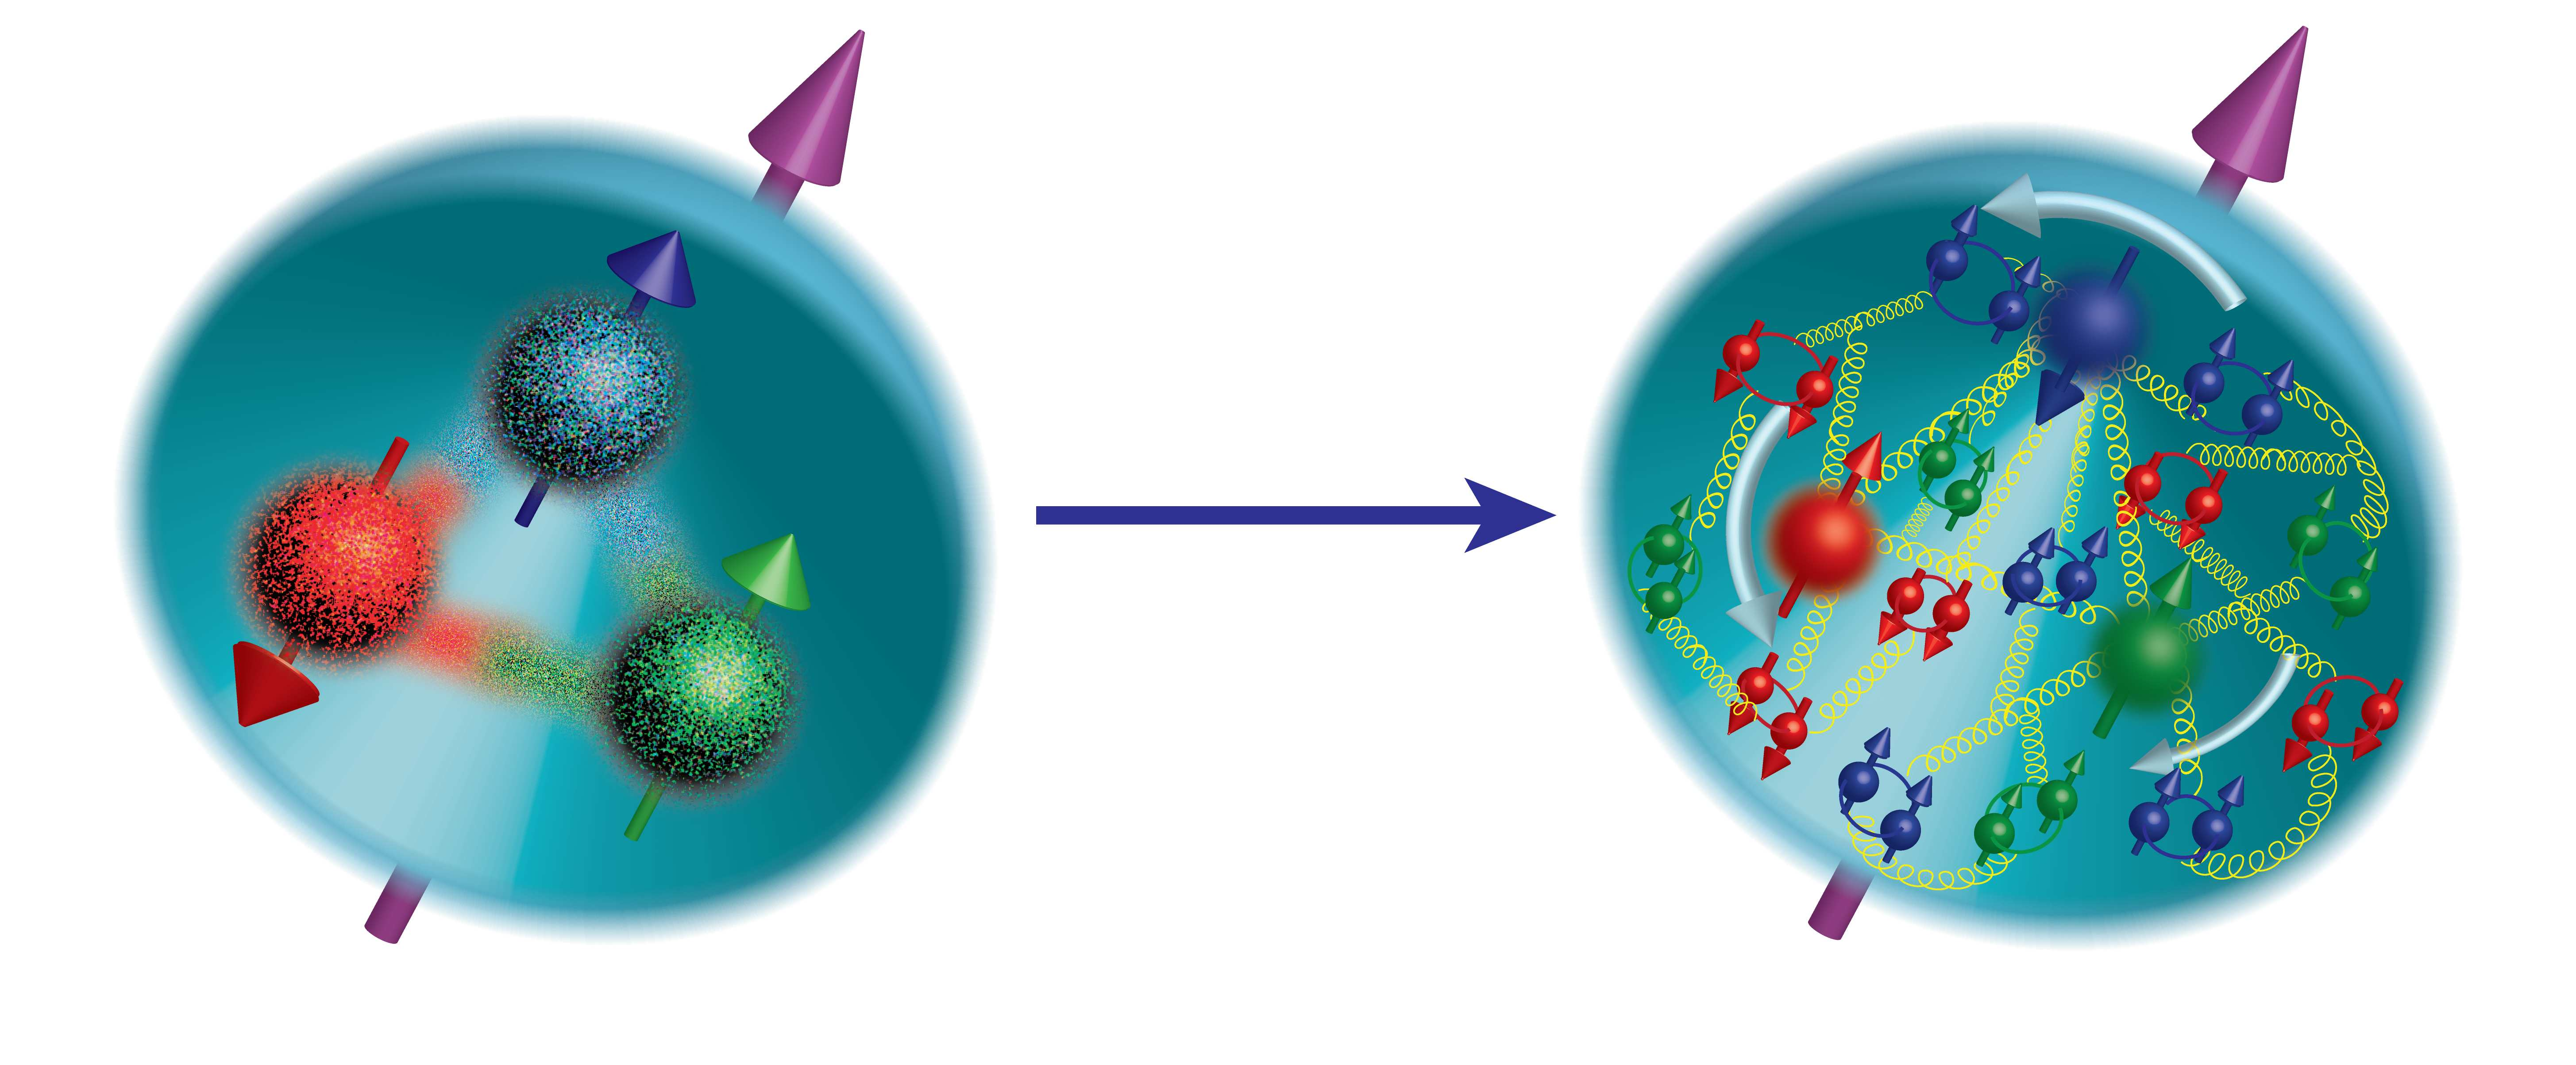
\includegraphics[scale=.08]{nucleon_spin.png}
	\caption[Evolution of our understanding of nucleon spin structure.]{Evolution of our understanding of nucleon spin structure. Left: In the 1980s, a nucleon’s spin was naively explained by the alignment of the spins of its constituent quarks. Right: In the current picture, valence quarks, sea quarks and gluons, and their possible orbital motion are expected to contribute to overall nucleon spin \cite{EICWhitePaper}.}
	\label{fig:nucleon_spin}
\end{figure}

\subsection{The EMC Effect}
It was first observed by the European Muon Collaboration (EMC), and confirmed by other experiments that there is a modification between the nucleon structure function, $F_2$, of deuterium to those of heavier elements as a function of Bjorken $x$ \cite{SRC_EMC_effect}. Figure \ref{fig:emc_effect} shows the ratios of the Deep Inelastic Scattering (DIS) cross sections of ${}^3$He (top) to Deuterium and ${}^4$He (bottom) to Deuterium as examples of this effect. Initial assumptions were that these cross section ratios would be unity, but measurements have clearly shown a suppression in this ratio for $0.3 < x < 0.8$, the now-called EMC Effect. One can also see an enhancement of the ratio for $0.1 < x < 0.3$ known as anti-shadowing, and the region of $x < 0.1$ where the ratio is again suppressed is the shadowing region.

\begin{figure}[!htb]
	\centering
	\includegraphics[scale=0.85]{EMC_He.png}
	\caption[Two examples of the EMC effect.]{Two examples of the EMC effect. Top: Ratios of ${}^3$He to Deuterium DIS cross sections from JLab (circles) and HERMES (triangles). Bottom: Ratios of ${}^4$He to Deuterium DIS cross sections from JLab (circles), SLAC (squares), and HERMES (triangles) \cite{EMC_Challenge}.}
	\label{fig:emc_effect}
\end{figure}

The reason for this modification to the DIS cross section is still a mystery, but the EIC hopes to shed light on this phenomenon by studying various coherent exclusive reactions, such as $J/\Psi$ production via $eA \rightarrow eAJ/\Psi$, which could allow for the quantification of initial conditions in heavy-ion collisions by mapping out the geometry of the nucleus in high-energy processes. This mapping can also help to understand other collective dynamics in inelastic collisions, such as the shadowing and anti-shadowing effects. where multiple nucleons interact coherently with the probe.

\subsection{Gluon Distributions Inside Nuclei}
As mentioned above, the EMC effect, the modification of the distribution of quarks in a nucleus versus their distribution in nucleons, is a known (yet still mysterious) phenomenon. It is suspected that this modification also occurs for gluons, with experiments such as ALICE showing evidence for gluon shadowing for $x \approx 10^{-3}$ \cite{ALICE_antishadowing}. The EIC hopes to measure this suppression of the structure functions thanks to its wider range of kinematics both in $x$ and $Q^2$, allowing not only for the measurement of gluon shadowing ($x < 0.05$), but also anti-shadowing ($x \approx 0.1$), and possibly the EMC effect for gluons ($x > 0.3$), shedding light on the origins of the EMC effect.

%----------------------------------------------------------------------
%	FACILITIES SECTION
%----------------------------------------------------------------------
\section{Facilities}
As of the writing of this thesis there are two competing designs for an EIC facility to be built in the United States: a figure-8 accelerator design for Thomas Jefferson National Accelerator Facility (JLab) (Figure \ref{fig:jleic_layout}), and a LINAC-ring (or ring-ring) accelerator design for Brookhaven National Lab (BNL) (Figure \ref{fig:erhic_layout}).

The JLab EIC (JLEIC) is planned to be approximately 1.4 km in circumference and have a footprint of roughly 500 m by 170 m. The design is a ring-ring with electrons and ions being stored in separate beam lines and collided at two interaction points  (IPs) (outlined in red in Figure \ref{fig:jleic_layout}) on the figure-8. The JLab CEBAF SRF linac will be used as an electron injector for electrons with 3 - 11 GeV/c momentum. The second ring will store an ion beam with momentum of 20 to 100 GeV/c for protons, up to 50 GeV/c per nucleon for light to medium mass N = Z nuclei, and up to 40 GeV/c per nucleon for heavy nuclei. The ion beams are generated and accelerated in a new ion injector complex with a LINAC plus figure-8 design that will be utilized to preserve ion polarization. The two main rings will be stacked vertically in the same underground tunnel \cite{JLEICdesign}.

The BNL facility, named eRHIC, will use a new electron beam facility based on an Energy Recovery LINAC that will be built inside of the Relativistic Heavy Ion Collider (RHIC) tunnel to collide with RHIC's pre-existing polarized proton/ion beam. The existing hadron ring will accelerate protons up to 250 GeV/c, $^3$He$^{+2}$ up to 167 GeV/c per nucleon, and heavier ions (e.g. gold or uranium) up to 100 GeV/c per nucleon. The new electron ring will be capable of producing electrons from 2 - 21 GeV/c \cite{eRHICdesign}. Figure \ref{fig:erhic_layout} shows the current design layout of the eRHIC facility (top) and the Brookhaven eA Solenoidal Tracker (BeAST) detector proposed for the interaction region (bottom).

%----------------------------------------------------------------------
%	PARTICLE ID SUBSECTION
%----------------------------------------------------------------------
\subsection{Particle Identification Requirements and Solutions}
The large center of mass energies and diverse physics program at an EIC necessitate a very sophisticated detector suite. The most basic process that the EIC will observe is inclusive DIS with nearly full reconstruction of the hadronic final state. The ability to accurately identify hadrons in the final state is therefore a key requirement for the physics program, as is shown by Figure \ref{fig:pythia_DIS} which shows the momentum distributions of pions and kaons for each region of interest for typical beam energies for both BNL and JLab.

As can be seen in Figures \ref{fig:jleic_layout} and \ref{fig:erhic_layout}, the layouts of the two detector concepts for JLab and BNL are slightly different, but the solutions for PID requirements are very similar. In the hadron endcap, because of the large final state energies the ideal PID detector would be a gaseous, mirror-based Ring Imaging Cherenkov (RICH) detector. This will provide $\pi/K/p$ separation up to 50 GeV/c momentum. The hadrons produced going towards the electron endcap scales in both energy and quantity with the energy of the electron beam energy. Although the maximum electron beam energies of JLab and BNL differ, PID up to 10 GeV/c momentum seems to be suitable for both facilities, and so a modular aerogel RICH detector is currently under development. In the central barrel region the necessary momentum coverage is not as high as that of the endcaps because the transverse momentum transfer from the electron beam to the ion beam is generally less than 10 GeV/c. This smaller momentum range coupled with a smaller space to fit a detector make a detector based on Detection of Internally Reflected Cherenkov light (DIRC) technology a desirable choice.

The design and prototype testing of components for a high-performance DIRC detector is the subject of this thesis and an ideal solution for PID in the EIC barrel region.


\begin{figure}[!htb]
	\centering
	\includegraphics[width=\textwidth]{JLEIC_layout3.jpg}
	\includegraphics[width=\textwidth]{JLEIC_detector.pdf}
	\caption[The top figure is a design of the EIC facility for JLab.]{The top figure is a design of the EIC facility for JLab. The two interaction points (IP) are highlighted in purple, and the current baseline design for the detector at the left-most IP is shown at the bottom \cite{eRD14}.}
	\label{fig:jleic_layout}
\end{figure}

\begin{figure}[!htb]
	\centering
	\includegraphics[width=\textwidth]{eRHIC_Layout.jpeg}
	\includegraphics[width=0.9\textwidth]{eRHIC_beast.pdf}
	\caption[The top figure is a design of the LINAC-ring option for an EIC facility at BNL.]{The top figure is a design of the LINAC-ring option for an EIC facility at BNL. The proposed BeAST (Brookhaven eA Solenoidal Tracker) detector is shown at the bottom \cite{eRD14}.}
	\label{fig:erhic_layout}
\end{figure}

\begin{figure}[!htb]
	\centering
	\includegraphics[width=0.72\textwidth]{pythia_DIS_regions.pdf}
	\caption[Momentum distributions for pions (red) and kaons (blue) in the electron endcap (top), barrel region (middle), and hadron endcap (bottom).]{Momentum distributions for pions (red) and kaons (blue) in the electron endcap (top), barrel region (middle), and hadron endcap (bottom). Plots were produced using the pythia simulation package for DIS events corresponding to collisions between 10 GeV electrons and 100 GeV protons, a common BNL/JLab kinematic, shown for a bin of $10<Q2<100\unit{GeV}^2$ \cite{eRD14}.}
	\label{fig:pythia_DIS}
\end{figure}
 % description of EIC and why it's needed

\chapter{DIRC Technology}
%----------------------------------------------------------------------
%	DIRC TECHNOLOGY CHAPTER
%----------------------------------------------------------------------
\label{ch:dirc}
DIRC detectors are based on the concept of the Detection of Internally Reflected Cherenkov light (DIRC) produced in a solid radiator (typically fused silica) to identify charged particles. It is a special type of Cherenkov counter, which uses the unique properties of Cherenkov radiation to separate charged particle species.

%----------------------------------------------------------------------
%	CHERENKOV RADIATION SECTION
%----------------------------------------------------------------------
\section{Cherenkov Radiation}
Einstein postulated in his Theory of Relativity that the speed of light in a vacuum, $c$, is the limit of the velocity of massive particles. In an optically transparent medium, however, the speed at which light propagates is modified: $c_{med} = c/n$, where $n$ is the index of refraction of the medium. Pavel Cherenkov discovered in 1934 that massive particles moving through a medium faster than the speed of light in that medium emit light in the form of now-called Cherenkov radiation. Cherenkov was able to establish several interesting properties of this radiation: it is only emitted from charged particles above a certain velocity threshold $v > c/n$, the intensity is proportional to the particle's path length, emission is prompt, and the light is polarized with a continuous wavelength spectrum. Later, in 1937, Ilya Frank and Igor Tamm theoretically formulated this radiation with fantastic agreement to Cherenkov's findings, and the three shared the 1958 Nobel Prize in Physics for their efforts \cite{CherenkovHistory}.

Further studies confirmed that Cherenkov radiation is emitted uniformly in azimuth ($\phi_c$) around the particle's direction of travel with the polar opening angle $\thetaC$ defined as

\begin{equation}
	\cos\thetaC = \frac{1}{\beta n(\lambda)},
	\label{eq:cherenkovformula}
\end{equation}

where $\beta = v_p/c$, $v_p$ is the particle's velocity, and the index of refraction is a function of the emitted photon wavelength. In a typical, dispersive optical medium the opening half-angle of the shock wave produced by the Cherenkov radiation, $\eta_C$ defined in Figure \ref{fig:cherenkovcone}, is not complementary to the Cherenkov angle. The relationship between the two is given by

\begin{equation}
	\cot\eta_C = \left[\frac{\diff}{\diff\omega}(\omega \tan\thetaC) \right]_{\omega_0} = \left[\tan\thetaC + \beta^2\omega n(\omega) \frac{\diff n}{\diff\omega}\cot\thetaC \right]_{\omega_0}
	\label{eq:openingangle}
\end{equation}
where $\omega_0$ is the central value of the considered frequency range. Because the second term in (\ref{eq:openingangle}) is zero only for non-dispersive media the shock wave front is not perpendicular to the Cherenkov cone in real detectors.

\begin{figure}[!htb]
	\centering
	\includegraphics[scale=1]{Cherenkov_cone.pdf}
	\caption[Illustration of the Cherenkov cone.]{Illustration of the Cherenkov cone \cite{ParticleDetectionHandbook}.}
	\label{fig:cherenkovcone}
\end{figure}

Because particles lose very little energy when radiating Cherenkov photons the emission is very weak. The number of photons $N_{photons}$ emitted per path length $L$ (in cm) by a moving particle with charge $z$ is given by the Frank-Tamm equation

\begin{equation}
	\frac{N_{photons}}{L} = \frac{\alpha^2 z^2}{r_e m_e c^2} \int \sin^2\thetaC (E) \diff E
	\label{eq:nphotons}
\end{equation}
%
where E is the photon energy in eV, the integral is taken over the region where $n(E)$ is greater than 1, $\alpha = \frac{1}{137}$ is the fine structure constant, $z$ is the projective charge in units of electron charge, and $\frac{\alpha^2}{r_e m_e c^2} = 370\unit{cm}^{-1}\unit{eV}^{-1}$.

%----------------------------------------------------------------------
%	APPLYING TO PID SECTION
%----------------------------------------------------------------------
\section{Applying the Cherenkov Effect to Particle ID}
In order to identify particle species one must know both the mass and charge of the particle in question. Because the Cherenkov angle encodes the particle's velocity it is, in principle, a simple matter to measure the particle's momentum with a tracking chamber as well as the velocity obtained from (\ref{eq:cherenkovformula}) to determine the mass and charge. Figure \ref{fig:angleseperation} shows how different particle species can be distinguished for a given momentum in fused silica.

Threshold counters are Cherenkov detectors used for particle identification (PID) by exploiting the fact that only particles above the threshold velocity $\beta > 1/n$ will emit Cherenkov photons. Therefore lighter particles will emit Cherenkov light while heavier particles will not for a given momentum.

\begin{figure}[!htb]
	\centering
	\includegraphics[width=\textwidth]{angle_seperation_enhance.pdf}
	\caption[Particle momentum (in GeV/c) versus Cherenkov angle (in mrad) for different particle species in fused silica ($n \approx 1.473$).]{Particle momentum (in GeV/c) versus Cherenkov angle (in mrad) for different particle species in fused silica ($n \approx 1.473$). While the full range (left) makes it seem as if separation between heavier species becomes more and more challenging, zooming in (right) shows that it is indeed to possible separate protons, kaons, and pions even at higher particle momentum.}
	\label{fig:angleseperation}
\end{figure}

%----------------------------------------------------------------------
%	RICH SECTION
%----------------------------------------------------------------------
\section{Ring Imaging Detectors}
Ring Imaging Cherenkov (RICH) detectors are designed to efficiently identify and separate different particle species over a wide range of momenta.

The information about a particle's velocity can be combined with momentum information from a tracking system to determine the mass as \cite{ParticleDetectionHandbook}

\begin{equation}
	m = \frac{p}{c} \sqrt{n^2 \cos^2\thetaC - 1}
	\label{eq:mass}
\end{equation}
%
A basic RICH system is shown in Figure \ref{fig:rich_basics}. A volume of radiator, either gaseous (e.g. $C_{4}F_{10}$) or solid (e.g. aerogel), is positioned upstream of an array of photosensors. A charged particle traveling through a thin radiator above the threshold velocity will continuously emit Cherenkov photons in a cone. The resulting image on the photosensor array is an annulus of thickness $d\tan\thetaC$ and an inner radius of $L\tan\thetaC$, where $d$ is the distance the particle traveled inside the radiator, $L$ is the distance between the radiator and the photosensors, and  $\thetaC$ is the usual Cherenkov angle (Figure \ref{fig:rich_basics}b). PID is done by measuring the average radius of the annulus and reconstructing the Cherenkov angle geometricly.

\begin{figure}[!htb]
	\centering
	\includegraphics[width=\textwidth]{RICH_rings.pdf}
	\caption[Basic concept of a proximity focusing Ring Imaging Cherenkov (RICH) detector (a), and an example of how they can be used to do PID based on particle mass (b).]{Basic concept of a proximity focusing Ring Imaging Cherenkov (RICH) detector (a), and an example of how they can be used to do PID based on particle mass (b) \cite{GregThesis}.}
	\label{fig:rich_basics}
\end{figure}


%----------------------------------------------------------------------
%	DIRC SECTION
%----------------------------------------------------------------------
\section{DIRC Detectors}
DIRC detectors work much the same way as a RICH in that they collect Cherenkov photons produced from a radiating material and use the created image on the photosensors to reconstruct the Cherenkov angle. In the case of a DIRC, the radiating medium is also used as a light guide as some of the Cherenkov photons undergo total internal reflection inside the radiator and are guided towards one end of the radiator to a readout (Figure \ref{fig:dircbasics}). The radiator of choice is a solid bar made of fused silica, with an index of refraction $n = 1.468$ at a photon wavelength of $\lambda = 420\unit{nm}$. A rectangular cross section and highly smoothed and polished sides ensure that the magnitude of the Cherenkov angle is preserved to within $<1$~mrad during internal reflection. Photons that are created propagating away from the readout are reflected back towards the readout by a mirror. Once the photons exit the radiator they are allowed to separate through an expansion volume before being imaged in both ($x, y$) position as well as time. The arrival position and propagation time of each detected photon are combined with tracking information to reconstruct the Cherenkov angle and determine the corresponding PID likelihoods (reconstruction methods and techniques for DIRC detectors will be discussed in detail in Chapter \ref{ch:analysis}).

\begin{figure}[!htb]
	\centering
	\includegraphics[scale=0.7]{DIRC_components.pdf}
	\caption[The basic components of a DIRC detector.]{The basic components of a DIRC detector. A solid radiator, typically fused silica (green); a mirror to redirect backward-going photons (pink); optional focusing optics (purple); an expansion volume to allow photons to separate in space (cyan); and a detector surface (brown) to record the position and arrival time of Cherenkov photons (blue).}
	\label{fig:dircbasics}
\end{figure}

The performance of a DIRC detector is given by the resolution in the Cherenkov polar opening angle of the particle track, $\sigma_{\thetaC,\text{track}}^2$, which can be written as:

\begin{equation}
	\sigma_{\thetaC,\text{track}}^2 = \sigma_{\thetaC}^2 / N_{\gamma} + \sigma_{\text{correlated}}^2
	\label{eq:performance}
\end{equation}
%
where $\sigma_{\thetaC}$ is the average single photon Cherenkov angle resolution, $N_{\gamma}$ is the number of measured photons per track, and $\sigma_{\text{correlated}}$ includes several correlated terms that contribute to the resolution such as the uncertainty in the particle track direction coming from external tracking systems, chromatic dispersion, and pixel size. Because the track direction is crucial to the reconstruction of the Cherenkov angle, this error needs to be small for the performance to not suffer. For the EIC a tracking resolution on the order of 1 mrad is required for adequate PID.

\begin{figure}[!htb]
	\centering
	\includegraphics[width=\textwidth]{BaBar_DIRC.png}
	\caption[Schematic of the BaBar DIRC and detection region.]{Schematic of the BaBar DIRC and detection region \cite{BaBarDIRC}.}
	\label{fig:babardirc}
\end{figure}

As of the writing of this thesis the only DIRC detector used in a full experiment is the BaBar DIRC at SLAC National Accelerator Laboratory, which was successfully operated from 1999 through 2008 \cite{BaBarDIRC}. It proved to be a robust, stable, and easy to operate system for more than 8 years, providing excellent pion/kaon separation for all tracks from $B$-meson decays. It used 4.9 m long radiator bars with a rectangular cross section of $17.25 \times 35 \unit{mm}^2$. Each bar was made of four $1.225\unit{m}$ long fused silica bars glued end-to-end. The bars were placed in 12 hermetically sealed containers, called bar boxes, each holding 12 radiator bars for a total of 144 bars. At the end of each box was attached a wedge of fused silica and a window to allow the photon image to expand before entering the water-filled expansion volume and being read out on one of 10,752 photomultiplier tubes (see Figure \ref{fig:babardirc}). Figure \ref{fig:babarperformance} summarizes the performance of the BaBar DIRC, showing excellent Cherenkov angle reconstruction (2.5 mrad, only 14\% larger than the design goal of 2.2 mrad) and photon yield per track.

\begin{figure}[!htb]
	\centering
	a)%
	\raisebox{-1.0\height}{\includegraphics[width=0.5\textwidth]{BaBar_SPR.png}}%
	b)%
	\raisebox{-1.0\height}{\includegraphics[width=0.5\textwidth]{BaBar_NPH.png}}
	\caption[Performance of the BaBar DIRC for $e^{+}e^{-} \rightarrow \mu^{+}\mu^{-}$ events.]{Performance of the BaBar DIRC for $e^{+}e^{-} \rightarrow \mu^{+}\mu^{-}$ events \cite{BaBarDIRC}. a) shows the difference between the measured and expected Cherenkov angle (dots) and a Gaussian fit to the data with a 2.5 mrad width (line). b) is the average number of detected photons vs. track polar angle for data (dots) and GEANT4 \cite{GEANT4} simulation (line).}
	\label{fig:babarperformance}
\end{figure}

\subsection{DIRCs in Future Experiments}
The BaBar DIRC has since inspired many other experiments/facilities, including the EIC, to utilize this new, novel PID system in a variety of ways (Figure \ref{fig:dirc_evolution}). The Focusing DIRC (FDIRC) proposed for the now-cancelled SuperB collider in Italy was the first to propose using some form of focusing for the Cherenkov photons, allowing for a factor of 10 smaller expansion volume \cite{FDIRC} \cite{FDIRC2}. The barrel DIRC for the PANDA experiment at FAIR in Germany will use shorter radiator bars for a more compact design \cite{PANDA_barrel}, while the PANDA disc DIRC will be used in the forward region and will be the first disc DIRC to be used in a high-performance $4\pi$ detector \cite{PANDA_disc}. Belle II at the SuperKEKB accelerator in Japan will utilize wide plates as radiators and focus on fast timing for PID in the barrel region \cite{Belle2_TOP}. The TORCH detector, similar to the PANDA disc DIRC, will be a large-area detector focusing on precision time-of-flight to do PID for low momentum kaons at the upgraded LHCb experiment \cite{TORCH}. The GlueX experiment at JLab will be recycling four bar boxes from the BaBar experiment to cover the forward region of their spectrometer; utilizing  focusing similar to the FDIRC design \cite{GlueX}.

\begin{figure}[H]
	\centering
	\includegraphics[width=\textwidth]{dirc_evolution.pdf}
	\caption[Evolution of the DIRC concept.]{Evolution of the DIRC concept. From top left to bottom right: BaBar Barrel DIRC \cite{BaBarDIRC}, Focusing DIRC \cite{FDIRC2}, PANDA Barrel DIRC \cite{PANDA_barrel}, PANDA Disc DIRC \cite{PANDA_disc}, Belle II Time of Propagation DIRC \cite{Belle2_TOP}, LHCb TORCH DIRC \cite{TORCH}, GlueX DIRC \cite{GlueX}, and the EIC DIRC.}
	\label{fig:dirc_evolution}
\end{figure}

%----------------------------------------------------------------------
%	RECONSTRUCTION SECTION
%----------------------------------------------------------------------
\section{Hit Patterns and Particle Separation Methods}
As mentioned previously, a DIRC detector is a compact RICH system that relies on internal reflection of the Cherenkov photons in the radiating material. However, as is illustrated in Figure \ref{fig:dircbasics}, not all of the light produced inside the radiator is internally reflected, as photons with an angle less than the critical angle (approximately $43^{\circ}$ for the interface from fused silica to air) with respect to the surface will escape the radiator. Because of this loss of photons the hit pattern of a DIRC is only roughly half of a typical RICH ring, which is then mirrored and folded in a complex way based on the shape of the expansion volume and where the photon exits the radiator. If the expansion volume is more radially compact the two ring segments become stacked side by side. To complicate matters further, if the expansion volume is small enough that reflections from the sides occur then the ring segments are folded on top of themselves to create much more complicated hit patterns. Figure \ref{fig:ring_comparison2} illustrates this folding of the hit pattern due to expansion volume size. Figure \ref{fig:prism_reflections} shows the contribution to the folded pattern from single reflections inside a prism shaped expansion volume.

Two approaches were used in the analysis presented in this thesis for particle species separation: reconstruction of the Cherenkov angle using a geometric reconstruction method similar to the one used by the BaBar DIRC, and time-based imaging using probability density functions (PDFs) \footnote{In this manuscript, 'PDF' refers to a 'probability distribution function' and does NOT refer to either an Adobe\textsuperscript{\textregistered} Portable Document Format or to a parton distribution function.} similar to that to be used by the Belle II imaging Time of Propagation (iTOP) counter.

\begin{figure}[H]
	\centering
	\includegraphics[scale=0.43]{ring_comparison2.pdf}
	\caption[Various detector geometries (left) and the resulting simulated hit patterns (right) from 1000 identical particles.]{Various detector geometries (left) and the resulting simulated hit patterns (right) from 1000 identical particles. A typical RICH detector (a), produces a very nice ring pattern. A DIRC detector with a sufficiently large expansion volume using a thin radiator bar (b) produces two ring segments. A DIRC with a radially compact expansion volume (c) will reflect one of the ring segments so that it will stack side by side. Finally, a DIRC detector with a compact expansion volume both radially and transversely (i.e. into and out of the page) (d) will cause the ring segments to fold in on themselves, making a fish-like pattern. The DIRC patterns are viewed from the back of the detector plane and rotated $90^{\circ}$ clockwise relative to the corresponding geometry.}
	\label{fig:ring_comparison2}
\end{figure}


\begin{figure}[H]
	\centering
	\includegraphics[width=\textwidth]{prism_reflections.pdf}
	\caption[For a prism-shaped expansion volume (a), different segments of the hit pattern correspond to different paths taken (b).]{For a prism-shaped expansion volume (a) \cite{GregThesis}, different segments of the hit pattern correspond to different paths taken (b). Paths with multiple reflections inside the prism (e.g. bottom-left) have been excluded for simplicity.}
	\label{fig:prism_reflections}
\end{figure}

\subsection{Cherenkov Angle Reconstruction}
The emission angle between a single photon and the particle track can be reconstructed from the observed photon coordinates on the detector plane. The spatial position of the centers of the radiator bar and the struck pixel are known and used to define the 3-dimensional unit direction vector $\vec{k} = (k_x, k_y, k_z)$ pointing from the center of the bar end to the center of the pixel (shown in Figure \ref{fig:k_vector}). The $k$-vector is defined as the photon exit vector just inside the bar. The direction vector from the bar center to the pixel center along with Snell's law are used to determine the $k$-vector. Excluding aberrations, any photon reaching this pixel originated with the same direction vector at the end of the bar, regardless of the photon origination point. Together with the particle direction $\vec{p} = (p_x, p_y, p_z)$ the Cherenkov angle for each photon can be calculated from

\begin{equation}
	\thetaC = \arccos\left(\frac{\vec{k}\cdot\vec{p}}{|p|}\right)
\end{equation}

\begin{figure}[!htb]
	\centering
	\includegraphics[width=0.65\textwidth]{k_vector.pdf}
	\caption[Schematic of the geometric reconstruction concept, with a photon (purple) being emitted from the particle track.]{Schematic of the geometric reconstruction concept, with a photon (purple) being emitted from the particle track. The direction of the k-vector can be used to determine the original direction vector, $\vec{k}_{org}$, of the photon and is used for the reconstruction of $\thetaC$ \cite{GregThesis}.}
	\label{fig:k_vector}
\end{figure}

In order to assign a value of the k-vector for each pixel a photon gun is used in GEANT4 to illuminate the detector plane. Roughly $10^5$ photons are created at the center of the bar near the bar/expansion volume interface uniformly in a solid angle of $~1.3\pi$ steradians and allowed to propagate through the expansion volume and onto the photosensors. The initial value of the k-vector, the propagation time,  number of bounces inside the expansion volume, and sensor and pixel number are all stored in a large table, called a lookup table (LUT). The values in the LUT are independent of particle species and momentum and only depends upon the detector geometry (e.g. the focusing optic, or the location of the bar relative to the expansion volume). Because of this a LUT for a given geometry can be generated before taking data. Another advantage to the geometric reconstruction is that a full simulation of the particle track is not needed which saves a lot of computation, as much of the computing power used during a simulation is used for the photon propagation through the bar.

Unfortunately, the direction of the k-vector as reconstructed by the pixel does not uniquely define the directionality of $\vec{k}_{org}$. Because the number of reflections inside the bar cannot be known there are 8 possibilities, or ambiguities, for the original directionality of the photon that must be considered (forward/backward, up/down, and left/right). Figure \ref{fig:bar_ambiguities} illustrates a 2D simplification of this problem, showing 4 possible photon directions propagating from the particle track. Here each of $\theta_{1-4}$ are possible values for the true Cherenkov angle. In the full 3D space this leads to up to 8 possibilities to be considered for the k-vector for each detected photon, and therefore up to 8 values of the Cherenkov angle $\thetaC$.

\begin{figure}[!htb]
	\centering
	\includegraphics[width=0.7\textwidth]{bar_ambiguities.pdf}
	\caption[2D illustration showing all possible combinations of k-vector directions off of the particle track.]{2D illustration showing all possible combinations of k-vector directions off of the particle track \cite{GregThesis}. Not shown are the additional 4 components where $k_x \rightarrow -k_x$.}
	\label{fig:bar_ambiguities}
\end{figure}

In addition to ambiguities coming from guessing the initial directionality of the k-vector inside the bar there are also ambiguities coming from the multiple possible paths that a photon could take from the center of the bar to a pixel inside the expansion volume. Figure \ref{fig:prism_ambiguities} shows a prism-shaped expansion volume, similar to that used in the analysis presented later in Chapter \ref{ch:analysis}, showing the labeling of the surfaces and an example of ambiguous photon paths from the bar to a pixel on the detector plane.

The number of ambiguous paths that are reconstructed can be reduced by averaging the initial direction of all photons in the LUT that have the same number and types of reflections and land in the same pixel. For a simplified example, see Figure \ref{fig:lut_averaging}

\begin{figure}[!htb]
	\centering
	\includegraphics[width=0.75\textwidth]{lut_averaging.pdf}
	\caption[A 2D example of averaging LUT entries to reduce prism ambiguity reconstructions.]{A 2D example of averaging LUT entries to reduce prism ambiguity reconstructions. The two photons reflecting off of the bottom prism face (blue) have been averaged to the one black photon. The two photons reflecting off of the top prism face (orange) have been average to the red photon. In this simplified example the number of entries in the LUT have been reduced by half. Angles have been exaggerated.}
	\label{fig:lut_averaging}
\end{figure}

The Cherenkov angle is not, however, only reconstructed for one photon, but for between 20 and 120 photons per particle track. For each photon at least one of these reconstructed $\thetaC$ values is correct, while the others contribute to a combinatorial background in a spectrum of the reconstructed angle, an example of which can be seen in Figure \ref{fig:combinatorial_background} for 7 GeV/c protons with a $125^{\circ}$ polar angle and made with an averaged path LUT.

\begin{figure}[!htb]
	\centering
	\includegraphics[width=\textwidth]{prism_ambiguities.pdf}
	\caption[Illustration of possible ambiguities in the $\thetaC$ reconstruction coming from possible paths in a prism-shaped expansion volume.]{Illustration of possible ambiguities in the $\thetaC$ reconstruction coming from possible paths in a prism-shaped expansion volume \cite{GregThesis}. Each face is labeled in a) along with an example of a direct path, while b) shows 3 possible paths that lead from the bar to a certain pixel: 1 top reflection (gold), 1 bottom reflection (blue), and 1 direct path (gray).}
	\label{fig:prism_ambiguities}
\end{figure}

\begin{figure}[!htb]
	\centering
	\includegraphics[width=\textwidth]{combinatorial_background.pdf}
	\caption[Simulated reconstructed Cherenkov angle per photon from a 7 GeV/c particle with a polar angle of $125^{\circ}$.]{Simulated reconstructed Cherenkov angle per photon from a 7 GeV/c particle with a polar angle of $125^{\circ}$. a) one photon from a proton with only bar ambiguities. b) all photons from one proton with only bar ambiguities. c) all photons from 1000 identical protons with only bar ambiguities. d) all photons from 1000 identical protons with both bar and prism ambiguities. e) same as d) but with constraints on the photon angle with the bar surface being greater than the critical angle for total internal reflections and neglecting y direction flips due to zero beam divergence. f) a zoom showing a buildup around the calculated value of 816 mrad along with a combinatorial background.}
	\label{fig:combinatorial_background}
\end{figure}

\subsection{Time-Based Imaging}
The other method of particle species separation that can be used for a DIRC is time-based imaging or time-based reconstruction, similar to that used by the Belle II Time-Of-Propagation counter. To do time-based reconstruction one must first generate a PDF of the timing information of each detector pixel for each value of particle species, momentum, polar track angle, and detector geometry (e.g. lens and bar types), thus giving a 5-dimensional function  of the timing distribution of photon hits \cite{PANDA_barrel}. Currently these PDFs cannot be computed analytically, so they are constructed computationally by either taking actual test beam data, or running simulations with sufficient statistics such that each pixel that can have a hit with the configuration of interest has a large enough occupancy to produce a more or less smooth PDF.

To reconstruct a data or simulation file using these PDFs the photon arrival time for each pixel with a recorded hit is compared to the PDF for each particle species, and the time-based likelihood of that hit corresponding to a given particle species $X$ is calculated as $L_{X} = \ln(h_{X})$, where $h$ is the value of the PDF for the given hit time. One can then do a pair-wise difference of these likelihood values (e.g. $L = L_{p} - L_{\pi}$) to build a log-likelihood distribution between two particle hypotheses and extract a separation power for particle identification. The separation power for time-based reconstruction between two particle species is given by the magnitude of the difference of the two log likelihood plots divided by the average sigma. An example of time-based reconstruction for a bar radiator with a prism expansion volume is shown in Figure \ref{fig:time-based_reco} for pions and kaons in a plate radiator with a prism expansion volume. This method of particle separation is also very useful for plate-type radiators as the LUTs in the geometric reconstruction assume the photons come from the center of the bar, which is no longer a good assumption for wide plates. 

\begin{figure}[!htb]
	\centering
	\includegraphics[width=\textwidth]{time-based_reconstruction.png}
	\caption[An example of time-based reconstruction for a plate radiator with a prism expansion volume for kaons (dashed) and pions (solid red).]{An example of time-based reconstruction for a plate radiator with a prism expansion volume for kaons (dashed) and pions (solid red). Photon arrival times for one MCP-PMT pixel are shown in a), and b) is the log-likelihood difference for kaon and pion hypotheses for multiple 3.5 GeV/c particles at $22^\circ$ polar angle \cite{PANDA_barrel}.}
	\label{fig:time-based_reco}
\end{figure}
 % explination of DIRC technology

\chapter{High-Performance DIRC@EIC}
%-------------------------------------------------------------------------------
%	DIRC@EIC CHAPTER
%-------------------------------------------------------------------------------
\label{ch:eicdirc}

%-------------------------------------------------------------------------------
%	DESIGN EVOLUTION SECTION
%-------------------------------------------------------------------------------
\section{Evolution of the DIRC@EIC Design}

%-------------------------------------------------------------------------------
%	CURRENT BASELINE DESIGN SECTION
%-------------------------------------------------------------------------------
\section{Current High-Performance DIRC Design}

%-------------------------------------------------------------------------------
%	SIMULATION SECTION
%-------------------------------------------------------------------------------
\section{Simulated Performance}

%-------------------------------------------------------------------------------
%	DESIGN OPTIMIZATIONS SECTION
%-------------------------------------------------------------------------------
\section{Potential Optimizations} % specifications of high-performance DIRC@EIC

\chapter{Testing DIRC Components}
%-------------------------------------------------------------------------------
%	DIRC TECHNOLOGY CHAPTER
%-------------------------------------------------------------------------------
\label{ch:components}
The validation of key components of the DIRC for an EIC in vital to show that the Geant4 simulation package produces results expected for the real detector. However, due to budget restraints it was not possible to build or otherwise procure a full scale prototype of the envisioned EIC DIRC discussed in Chapter \ref{ch:eicdirc} (e.g. $2\unit{mm}$ pixel MCP-PMTs are not available on the market). Instead a series of test bench measurements were made for both the NLaK33 material of the 3-layer lens and for the performance of similar MCP-PMTs in high magnetic field environments.
The FDIRC R\&D program found that implementing focusing into the design of a DIRC improves performance and allows for a smaller, more compact expansion volume. A DIRC at EIC hopes to take advantage of this by utilizing a new 3-layer spherical lens design, a schematic of which is shown in Figure \ref{fig:3CS_schematic}a. 

\begin{figure}[ht]
	\centering
	\includegraphics[width=\textwidth]{3CS_schematic.pdf}
	\caption{Schematic drawing of the 3-layer lens design with two layers of fused silica sandwiching a layer of high refractive index NLaK33 glass (a), and a side and front view of a prototype lens built for testing (b).}
	\label{fig:3CS_schematic}
\end{figure}



%-------------------------------------------------------------------------------
%	3-LAYER LENS OPTICS SECTION
%-------------------------------------------------------------------------------
\section{Optical Properties of 3-Layer Lens}


%-------------------------------------------------------------------------------
%	NLAK33 RAD HARDNESS SECTION
%-------------------------------------------------------------------------------
\section{Radiation Hardness of NLaK33 Material}

%-------------------------------------------------------------------------------
%	HIGH-B TESTS SECTION
%-------------------------------------------------------------------------------
\section{Performance of MCP-PMTs in High Magnetic Field} % testing lens focal plane and rad hardness, and MCP-PMTs

\chapter{3-Layer Lens Performance in A Particle Beam}
%----------------------------------------------------------------------
%	CERN TEST BEAM CHAPTER
%----------------------------------------------------------------------
\label{ch:analysis}

Along with determining the focal plane and radiation hardness of the 3-layer lens design, another crucial step towards solidifying an EIC DIRC design was to test the new lens in a prototype DIRC with a real particle beam. Because not all of the components of the high-performance DIRC baseline design for an EIC are currently available it is necessary to validate the simulation package currently used to design and optimize the system. In June and July of 2015 the PANDA Barrel DIRC group along with myself and Dr. Grzegorz Kalicy from CUA conducted a test beam at the European Organization for Nuclear Research (CERN) with a prototype DIRC for the PANDA experiment. This was used as an opportunity to evaluate the performance of the 3-layer lens in a real particle beam. The beam was a hadron-rich beam with momentum tunable from 1 - 10 GeV/c. A standalone GEANT4 simulation package developed for the PANDA DIRC prototype (and later modified for the EIC DIRC geometry) was used for look-up table (LUT) generation, data monitoring, and comparison to data.
%The EIC DIRC simulation package was modified to use this new geometry setup so that data could be compared to simulation. 
The two most important quantities measured during this test beam were the photon yield per track and the Single Photon Resolution (SPR). Verifying these measurements with simulation give a good indication that the performance shown in Chapter \ref{ch:eicdirc} is what should be reasonably expected from a real EIC DIRC detector.

%----------------------------------------------------------------------
%	PROTOTYPE SETUP SECTION
%----------------------------------------------------------------------
\section{2015 Test Beam Prototype Setup}
The PANDA prototype was situated in the CERN Proton Synchrotron (PS) T9 experimental hall \cite{CERN_T9}. A 200 mm thick aluminum target upstream of the T9 hall was used to produce a hadron-rich beam comprised mostly of protons, pions, muons, and electrons with a very small amount of kaons. A series of dipole and quadrupole magnets allowed for steering and focusing of the beam, as well as selecting specific particle momenta in the range of 1 to 10 GeV/c for data taking. A scintillator monitored the intensity of the beam and a wire chamber monitored the x/y profile at the exit of the beam pipe.

\begin{figure}[!htb]
	\centering
	\includegraphics[width=\textwidth]{testbeam_2015.pdf}
	\caption{CAD drawing of the T9 experimental hall with the PANDA DIRC prototype setup. Two time-of-flight (TOF) detectors were separated by 29 m and used for proton/pion separation. Two trigger systems were used for the start and stop times of the readout electronics.}
	\label{fig:testbeam_2015}
\end{figure}

A CAD drawing of the experimental setup in the T9 hall can be seen in Figure \ref{fig:testbeam_2015}. The DIRC prototype was situated between two time-of-flight (TOF) detectors that were spaced 29 m apart to tag protons and pions. Figure \ref{fig:TOF_PID} shows the time-based separation of different particle species for 4 different beam momenta. Two scintillator counters (named Trigger 1 and Trigger 2) were placed in front of and behind the prototype. A coincidence of the trigger signals was used as the DAQ event recording trigger. Two veto counters were also set up between the two TOF detectors to reject background particles that strayed significantly from the beam path.

\begin{figure}[!htb]
	\centering
	\includegraphics[width=0.85\textwidth]{TOF_PID.png}
	\caption{Time-of-flight (TOF) particle tagging for 3, 5, 7, and 10 GeV/c beam momentum with a 29~m separation between TOF stations (MCP2 and SciTil1) each with between 50-80~ps time resolution. As a side note: it is immediately obvious that a simple TOF system as a solution to PID in the limited space of the barrel region of an EIC is infeasible as even at 5 GeV/c momentum the signal between pions and kaons are difficult to separate, and at 10 GeV/c it is neigh-impossible even with a 29~m separation between stations. }
	\label{fig:TOF_PID}
\end{figure}

\begin{figure}[!htb]
	\centering
	\includegraphics[width=0.6\textwidth]{PANDA_prototype2.pdf}
	\caption{CAD drawing of the 2015 PANDA DIRC prototype setup. The radiator (1), optics (2), expansion volume (3), $3\times5$ array of MCP-PMTs (4), readout (5), and TRB units (6) are supported by an aluminum frame that can move in two directions and rotate, as indicated by the red arrows.}
	\label{fig:PANDA_prototype}
\end{figure}

Figure \ref{fig:PANDA_prototype} shows a CAD drawing of the prototype setup. The prototype was held in place by a custom-built aluminum support structure with rails and a rotating table that allow the detector to be translated and rotated relative to the beam. The rotation of the prototype was verified using a remotely operated motor and camera. The radiator was carefully held in place by two aluminum braces equipped with three micrometer screws which allowed for fine adjustments in the position of the bar. Alignment of all components in the beam line were done with a GLL2-80 Dual Plane Leveling and Alignment Laser by Bosch \cite{BoschLaser}, which provides both vertical and horizontal self-leveled planes. An example of alignment of a radiator plate is shown in Figure \ref{fig:testbeam_alignment}. 

\begin{figure}[!htb]
	\centering
	\includegraphics[width=0.8\textwidth]{testbeam_alignment.JPG}
	\caption{Plate radiator being adjusted by micrometer screws using the Bosch Dual Plane Laser as a guide. When the light reflected off of the radiator lined up with the incoming beam from the laser on the white paper in both the horizontal and vertical directions the radiator was aligned with the beam line.}
	\label{fig:testbeam_alignment}
\end{figure}

\begin{figure}[!htb]
	\centering
	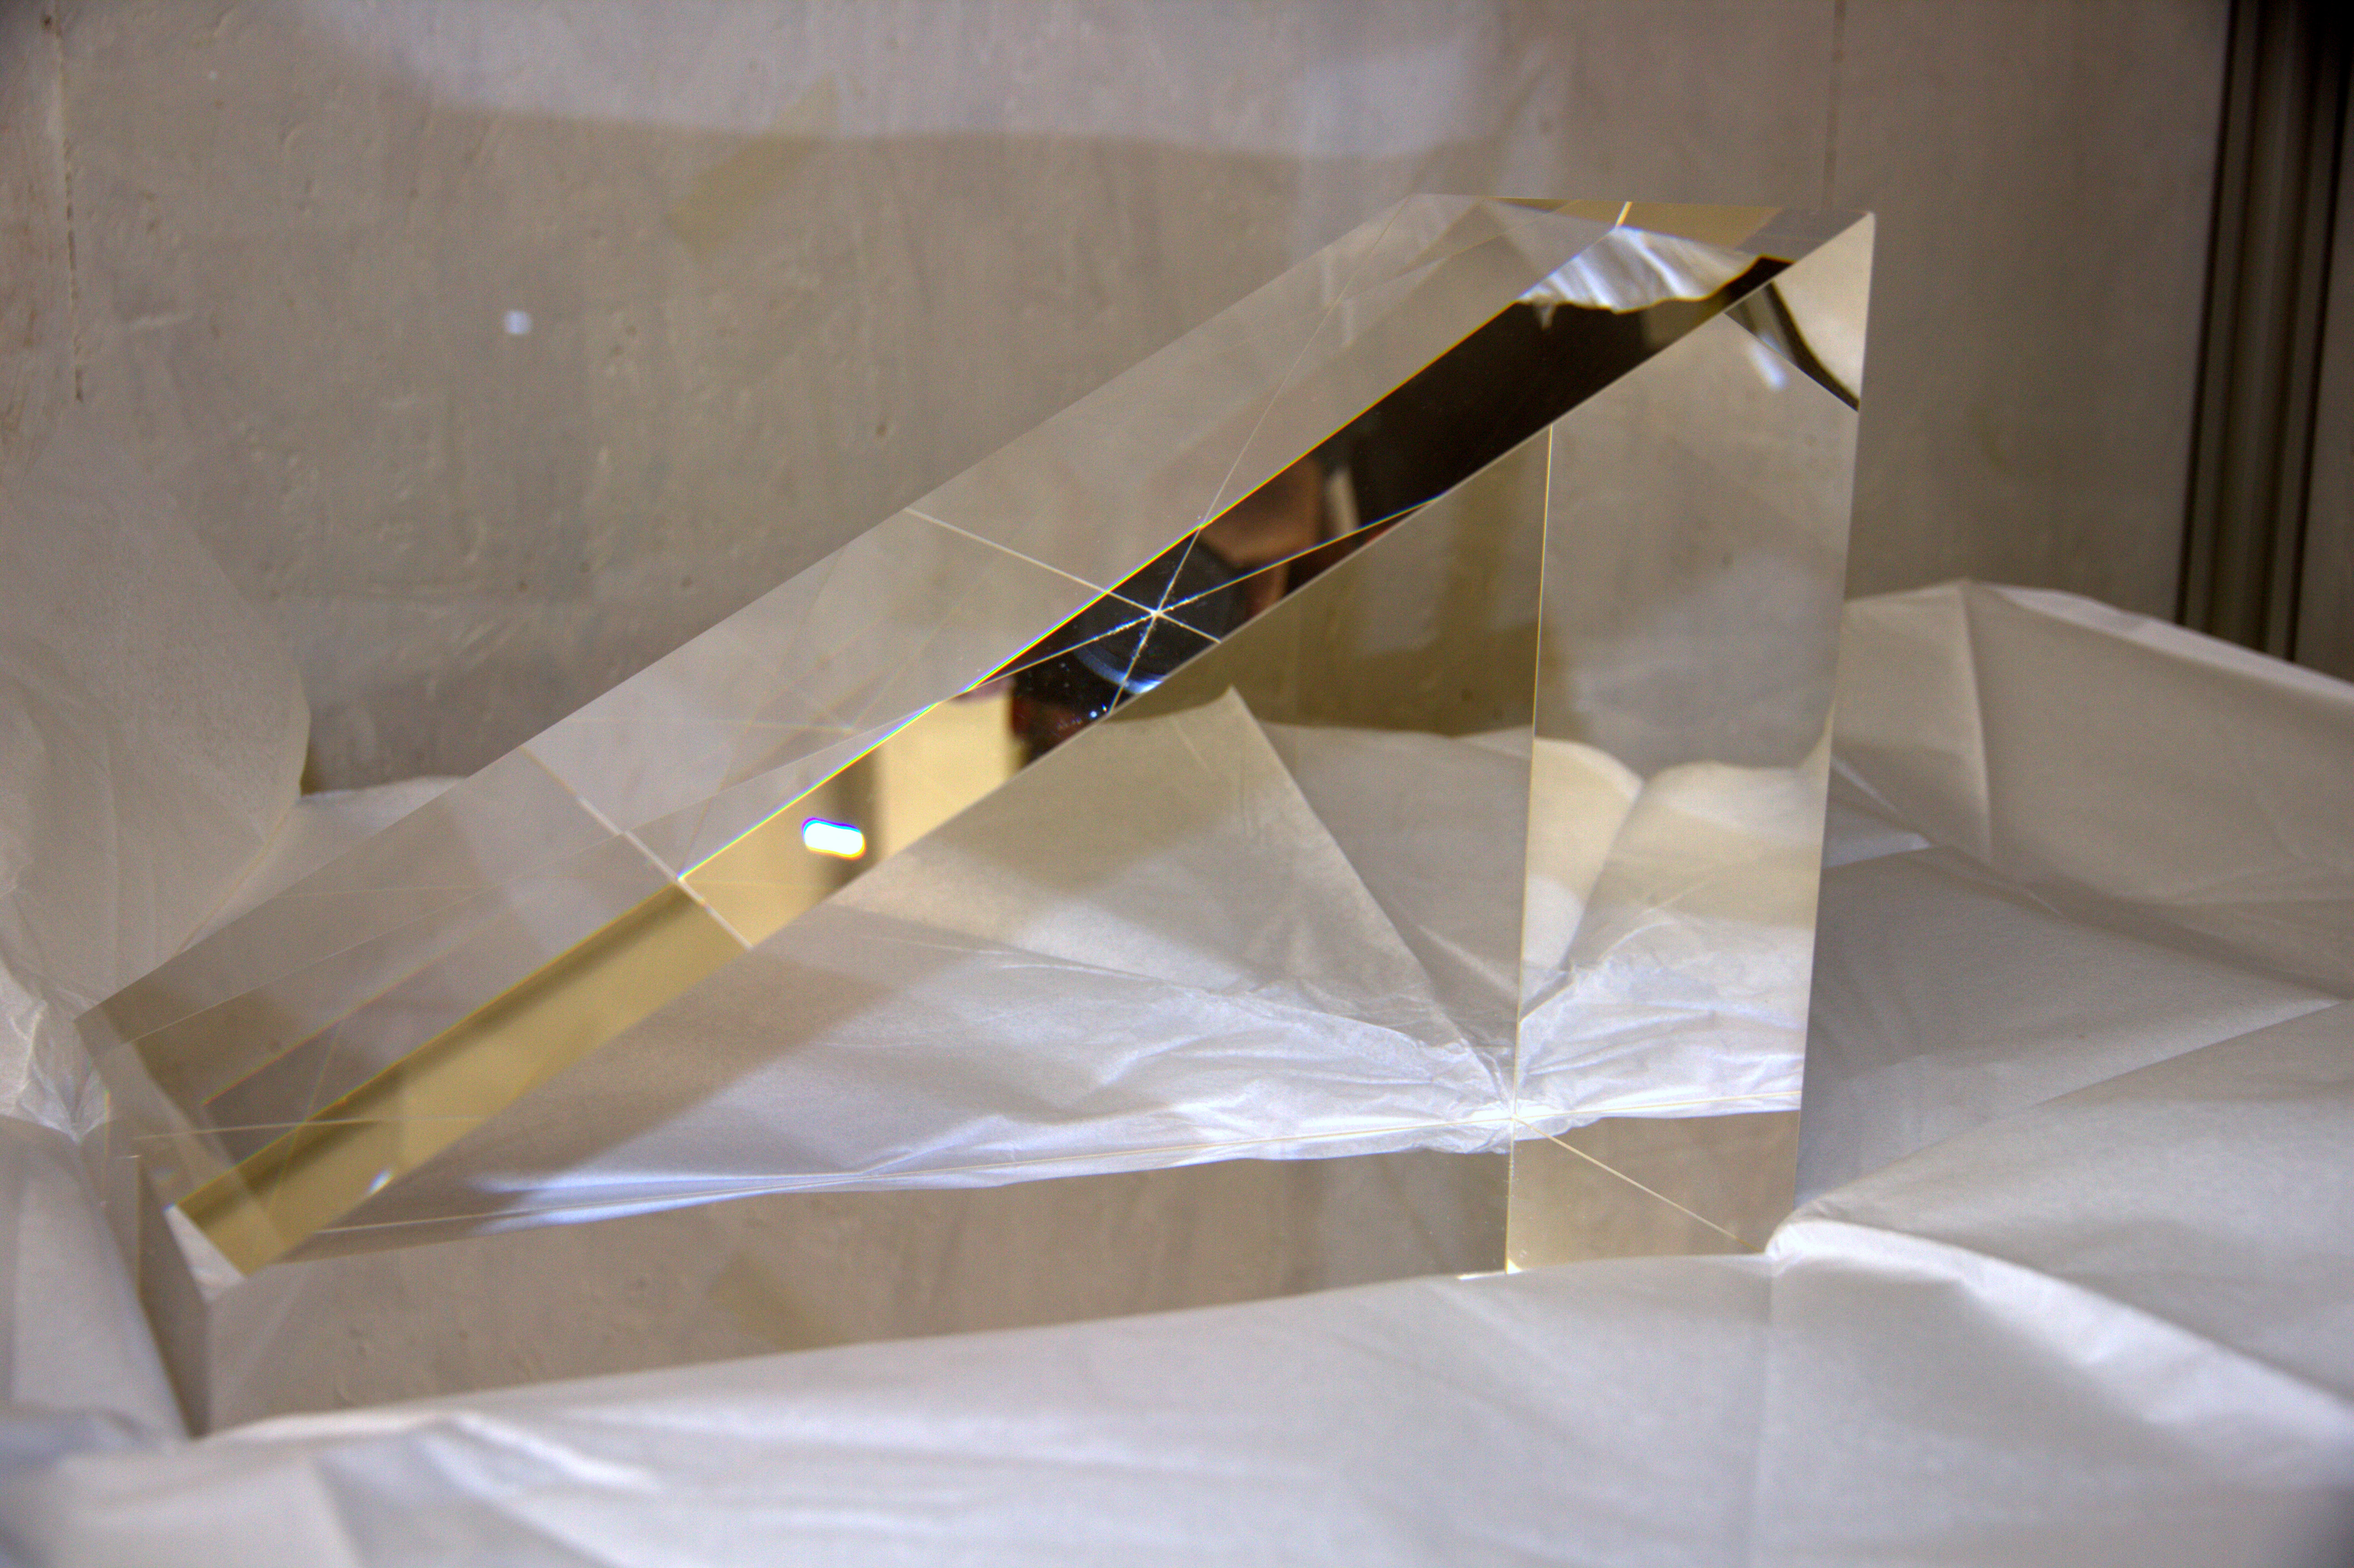
\includegraphics[width=0.7\textwidth]{30-deg-prism.pdf}
	\caption{Picture of the $30^{\circ}$ prism expansion volume used in the 2015 test beam.}
	\label{fig:prototype_prism}
\end{figure}

The optical component is attached to one end of the bar and a mirror is attached to the other. A compact prism expansion volume with dimensions $50\times170\times300\unit{mm}^3$ and an opening angle of $30^\circ$ (shown in Figure \ref{fig:prototype_prism}) was attached to the optical component (except in the case of an air-gap lens). A $3\times5$ array of PHOTONIS Planacon XP85102 MCP-PMTs with a total of 960 pixels ($6\times6\unit{mm}^2$ each) were held in place by a support structure and coupled to the expansion volume. The MCP-PMTs were read out by a DAQ system based on the trigger and readout board (TRB3) and the PADIWA discriminator card \cite{PANDA_electronics}. Couplings between the bar/lens, lens/prism, and prism/MCP-PMTs were done using Eljen EJ-550 optical grease \cite{EljenTech}. The mirror was not coupled directly to the bar, but held in place flat against the bar in order to prevent slight variations in grease thickness from effecting the angle of reflection.

The discriminating threshold signals for each MCP-PMT was adjusted and the difference between the discriminator and trigger signals were recorded by the TRB system. Noise events such as photons from delta electrons in the radiator bar and dark noise from the detectors were cut out using this timing information. Some channels had a very large background count rate and were masked. Calibration of the timing resolution of each channel was done using a 405 nm Picosecond Injection Laser (PiLas) PiL040SM by Advanced Laser Diode Systems \cite{PiLas} and a 660 nm Picosecond Pulsed Diode Laser (PDL 800-D) by PicoQuant \cite{PicoQuant}. The laser pulses were connected to an opal glass diffuser to illuminate the entire MCP-PMT plane. Calibrations were performed both daily and any time the geometric configuration was changed.

Data were taken for approximately 30 days, accumulating roughly 500 million triggers. Both bar and plate radiator geometries were tested with several optical components. Scans in polar angle between $20^\circ$ and $150^\circ$ were taken for many configurations. Scans in momentum up to 10 GeV/c were taken for select angles and geometries. As this was an opportunistic run for the EIC group, data taking was based on the needs of the PANDA DIRC group. They require separation power information for pion/kaon at 3.5 GeV/c, but since the T9 beam had a very small amount of kaons it was decided to instead study pion/proton separation at 7 GeV/c as the difference in Cherenkov angle for both cases is roughly 8 mrad. The results presented below will be from data taken with a bar radiator, 3-layer spherical lens, 7 GeV/c hadron-rich beam, and polar angles from  $20^\circ$ - $150^\circ$.

%----------------------------------------------------------------------
%	SIMULATION SECTION
%----------------------------------------------------------------------
\clearpage
\section{Prototype Simulation}
The accurate recreation of a DIRC detector in simulation is crucial for data analysis as it allows for the generation of the look-up-tables (LUTs) for geometric reconstruction, as well as a reference for the hit patterns \footnote{For the purposes of this document a ``hit" or ``photon" refers to a signal from a single pixel in an MCP-PMT. However because of an irreducible background it cannot be said for certain which signals are from true Cherenkov photons. What is truely measured are photo-electrons.} of the real-time monitoring system in the case of the 2015 CERN test beam campaign. A standalone GEANT4 simulation package was used for the CERN test beam, from which the EIC DIRC simulation in Chapter \ref{ch:eicdirc} was produced. Material properties for fused silica, NLaK33, the mirror, the optical grease, and the MCP-PMTs were included. The timing resolution of the simulation was based on findings of the laser calibration data and set to be 200 ps. For each configuration of the prototype the geometry for each element (e.g. relative positioning for the bar to the lens and prism) were adjusted to the values carefully measured while changing configurations.

\begin{figure}[!htb]
	\centering
	\includegraphics[width=\textwidth]{MCP_QE_2015.png}
	\includegraphics[width=\textwidth]{Photonis_QE.png}
	\caption{Channel-by-channel map of the relative quantum efficiency (QE) of each $6\times6\unit{mm}^2$ pixel of each MCP-PMT (64 pixels per MCP-PMT) used in the simulation of the 2015 test beam prototype (top). Absolute QE values in the simulation are the product of the channel-by-channel values with the wavelength dependent QE of a Planacon XP85012 MCP-PMT (bottom).}
	\label{fig:quantum_efficiency}
\end{figure}

Also included in the simulation is the quantum efficiency (QE) of the MCP-PMTs. Each MCP-PMT was scanned for QE and gain uniformity with a 372 nm laser pulser at Erlangen University. The mappings of QE were normalized to MCP-PMT 10 (when counting from bottom to top and left to right, starting at 0) and used as relative QE maps in the simulation (Figure \ref{fig:quantum_efficiency} top). To get the absolute QE for each pixel a scan was done of the QE as a function of photon wavelength (Figure \ref{fig:quantum_efficiency} bottom). The QE in the simulation was calculated by multiplying the relative QE of each pixel by the QE corresponding to the wavelength of the photon being detected by the pixel in the simulation.

\begin{figure}[!htb]
	\centering
	\includegraphics[width=0.7\textwidth]{proton_track_example.pdf}
	\caption{a) shows a visualization of the GEANT4 simulation of a single 7 GeV/c proton (red) traveling through the 2015 prototype with a bar radiator at a polar angle of $125^{\circ}$, b) is the accumulated hit pattern of 10,000 identical protons from simulation, and c) is the accumulated hit pattern of 10,000 tagged proton tracks from test beam data at 7 GeV/c beam and $125^{\circ}$ polar angle.}
	\label{fig:proton_track_example}
\end{figure}

Figure \ref{fig:proton_track_example}a shows an example of one simulated proton track with 7 GeV/c momentum (red) at a polar angle of $125^{\circ}$ traversing a bar radiator with the 3-layer lens focusing, and producing Cherenkov photons (yellow). Figure \ref{fig:proton_track_example}b is the accumulated hit pattern on the MCP-PMTs of 10,000 identical protons with the same configuration as in (a). Figure \ref{fig:proton_track_example}c is the accumulated hit pattern of 10,000 tagged proton events in the test beam data with 7 GeV/c beam momentum, $125^{\circ}$ polar angle, and the bar radiator and 3-layer lens configuration. The simulation very nicely reproduces the test beam hit pattern, giving a good indication that the simulation has the proper positioning of all the components.

%----------------------------------------------------------------------
%	DATA ANALYSIS SECTION
%----------------------------------------------------------------------
\clearpage
\section{Data Analysis}
Several studies were done during the CERN 2015 test beam campaign using both a radiator bar and plate, five different focusing configurations, and a range of momentum. Some studies were used as test runs for calibration and debugging. Information on the main data studies are shown in Table \ref{tab:runs2015}.

\begin{table}[]
\centering
\caption{Studies made during the 2015 CERN test beam campaign, including geometric configuration, momentum, and number of data points taken.}
\label{tab:runs2015}
\begin{tabular}{ccccc}
Study ID & Radiator & Lens & Momentum (GeV/c) & Data points \\
150 & bar & 2-layer spherical & 7 & 34 \\
151 & bar & 3-layer spherical & 7 & 46 \\
152 & plate & no lens & 7 & 28 \\
153 & plate & 2-layer cylindrical & 7 & 29 \\
154 & bar & 1-layer air gap & 7 & 44 \\
155 & bar & 1-layer air gap & 7 & 17 \\
157 & bar & 2-layer cylindrical & 7 & 43 \\
158 & bar & 3-layer spherical & 7 & 15 \\
159 & bar & no lens & 7 & 28 \\
160 & bar & 3-layer spherical & 5 & 47 \\
161 & plate & no lens & 5 & 29 \\
162 & plate & 2-layer cylindrical & 5 & 29 \\
170 & bar & 3-layer spherical & momentum scan & 9 \\
171 & plate & no lens & momentum scan & 8 \\
173 & plate & 2-layer cylindrical & momentum scan & 8 \\
174 & bar & 1-layer air gap & momentum scan & 8 \\
179 & bar & no lens & momentum scan & 9 \\
\end{tabular}
\end{table}


Two studies were chosen for the analysis in this thesis based on geometric configuration (bar and 3-layer lens) and momentum (7~GeV/c): 151 and 158. Study 151 is the primary data set because of its larger range in polar angle, while study 158 is used for comparison and error evaluation. Each data set represents approximately 1 day of beam.

\subsection{Event Selection}
The prototype data taken were stored in the list mode data format of the HADES DAQ system prototcol \cite{HADES_DAQ} and converted offline into the CERN ROOT data format \cite{ROOT} for analysis. The DAQ was started by a signal from Trigger 1, and events were required to have signals in Trigger 1, Trigger 2, and both TOF counters to ensure a well-defined beam spot and valid $\pi/p$ tagging from the TOF system. The veto counters were also required in event selection, but later found to be unnecessary for constraining the beam spot.

Hits were selected in a time window of $\pm 40$ ns relative to the Trigger 1 time. Channels with large electronics noise above 1 MHz and one defective PADIWA card were masked, with the same masking scheme applied to the simulation. Events with 5 or fewer MCP-PMT hits were also excluded from reconstruction due to lack of statistics for the reconstruction. It is also worth noting that, though the QE of the MCP-PMTs is more or less uniform, MCP-PMTs 12, 13, and 14 had poor performance during the test run due to electronics issues.

As mentioned previously the timing difference between the two TOF stations allowed for tagging an event as either pion or proton. Figure \ref{fig:tof_timing} shows the TOF time distributions for 5 GeV/c (top) and 7 GeV/c (bottom) beam momenta. These distributions were fitted with Gaussian functions near the proton and pion peaks and a $\pm2\sigma$ window around the peaks was used for selection (dashed lines).

\begin{figure}[!htb]
	\centering
	\includegraphics[width=\textwidth]{TOF_timing.pdf}
	\caption{Time difference between the two TOF stations for beam momenta of 5 GeV/c (top) and 7 GeV/c (bottom). The peaks were fitted and a $\pm2\sigma$ selection window was taken (dashed lines).}
	\label{fig:tof_timing}
\end{figure}

The timing of the hits in the MCP-PMTs were also constrained. Based on the orientation of the detector in the beam the time for the photon to propagate can be calculated based on the total bar path traveled ($Z$), using Figure \ref{fig:time_difference}a and
\begin{equation}
\begin{split}
	Z &= 
	\begin{cases}
		z_0 + \Delta z  & \text{direct photons} \\
		2L - z_0 - \Delta z  & \text{reflected photons}
	\end{cases}
	\\
	\Delta z &= -\cot(\alpha) \times \left[ D_2 + D_1\times\cot\left( 135 - \frac{\alpha}{2} \right) \right]
\end{split}
	\label{eq:time_diff_prop}
\end{equation}
%
where $L$ is the total length of the radiator, $z_0$ is the nominal perpendicular distance between the particle beam and the end of the radiator, $D_1$ is the distance from the pivot point of the radiator to the particle beam, $D_2$ is the distance from the pivot point to the radiator, and $\alpha$ is the polar angle.
Comparing the difference between the calculated expected arrival time and the actual arrival time of the photons gives a time difference distribution, shown in Figure \ref{fig:time_difference}b. In simulation it is to possible to exclude times associated with incorrect reconstructed paths from the LUT. Using this time distribution from only correct simulated paths it was determined that a time difference cut of $\pm1$~ns was sufficient across all polar angles for geometric reconstruction.

\begin{figure}[!htb]
	\centering
	\includegraphics[width=\textwidth]{time_difference.pdf}
	\caption{a) Illustration showing how total bar path length ($Z$) is calculated for the expected arrival time of photons based on distances from the pivot point (cyan circle) and particle beam ($D_1$),the pivot point to the radiator ($D_2$), nominal perpendicular distance between the beam and the end of the bar ($z_0$), and the polar angle ($\alpha$). Note that in the case of b) Example time difference distribution of experimental data (black), full simulation (red), and simulation including only correct prism paths from the LUT (blue) for $125^\circ$ polar angle. The dashed lines indicate the $\pm$1~ns cut taken during analysis. }
	\label{fig:time_difference}
\end{figure}


\subsection{Geometric Reconstruction}
The geometric reconstruction for the CERN 2015 test beam data was done in much the same manner as that described in Chapter \ref{ch:eicdirc}, however, three corrections were applied to the test beam data to improve resolution and overall performance: a correction to account for charge sharing between pixels in the MCP-PMTs, a per-MCP-PMT correction to the reconstructed mean $\thetaC$ for each polar angle, and a subtraction of the simulated path ambiguity background from beam data. Evaluation of the statistical and systematic uncertainties was also done for both simulation and beam data. Fitting of the main peak of the reconstructed Cherenkov angle was done in the same manner for both test beam data and simulation. Detailed information about the fitting for both protons and pions can be seen in Table \ref{tab:fitting_info} of Appendix \ref{appendix:fitting}. Results for photon yield, SPR, and reconstructed mean $\thetaC$ are presented below.

\subsubsection{Charge Sharing Correction}
It was discovered that many events in the prototype data showed multiple adjacent MCP-PMT pixels firing in a single event. It is difficult to say with certainty if neighboring firing pixels, such as the example shown in Figure \ref{fig:charge_sharing}a, fired independently or if charge sharing between the pixels occurred, effectively spreading the pixel's signal across multiple pixels. Because the width of each pixel corresponds to roughly a 20~mrad spread in Cherenkov angle the results of reconstructing these clustered pixels with the standard averaged LUT resulted in wider than expected reconstructed Cherenkov angle distributions for the prototype data. 

The solution was to modify the LUT to reconstruct the position of the photon not from the center of each pixel, but towards an edge, weighted by the position of neighboring firing pixels. Each pixel is subdivided into 9 sections in the LUT, as in Figure \ref{fig:charge_sharing}b. The reconstruction algorithm first determines if and where adjacent firing pixels are located for each hit and then reconstructs the Cherenkov angle at the center of the section most heavily weighted. Figure \ref{fig:charge_sharing_reco} shows the effect of this charge sharing correction for simulation (top) and experimental data (bottom) at $90^\circ$ polar angle. As was expected, the simulation, which does not include charge sharing, was largely unaffected. In the prototype data, however, the correction served to narrow the reconstructed Cherenkov angle peak and reduce background contributions.

\begin{figure}[!htb]
	\centering
	\includegraphics[width=\textwidth]{charge_sharing.pdf}
	\caption{a) A zoomed in view of a single MCP-PMT showing an example hit pattern from a single particle track. The 3 isolated pixels (red) have no neighboring hits. The 3 clustered hits (green), however, are adjacent to other firing pixels and thus it is hard to determine with timing alone if these are the result of a single photon from the bottom right pixel that resulted in charge sharing, 3 independent photons hitting all 3 pixels, or some combination of 2 photons hitting 2 of the pixels that resulted in charge sharing. To compensate for this uncertainty each pixel is subdivided, as in (b), into 9 regions such that the LUT will reconstruct the photon angle from different areas of the pixel. For the case of (a) the top pixel in the cluster would be reconstructed from point 7, the bottom left pixel from point 5, and the bottom right pixel from point 2, while the 3 isolated pixels would all be reconstructed from point 0.}
	\label{fig:charge_sharing}
\end{figure}

\begin{figure}[!htb]
	\centering
	\includegraphics[width=\textwidth]{chargeshare_90_sim.png}
	\includegraphics[width=\textwidth]{chargeshare_90_data.png}
	\caption{Reconstructed Cherenkov angle of 7 GeV/c protons for simulation (top) and prototype data (bottom) for $90^\circ$ polar angle using the standard LUT (blue) and the charge-sharing-corrected LUT (red). The simulation is largely unaffected, while in the data the peak has been narrowed and the background reduced.}
	\label{fig:charge_sharing_reco}
\end{figure}


\subsubsection{Per-MCP-PMT $\theta_{C}$ Correction}
The fitted mean of the reconstructed Cherenkov angle from geometric reconstruction showed a non-constant value across the prototype polar angle range for both simulation and experimental data. To correct for this non-constant shift a per-MCP-PMT $\thetaC$ correction was implemented in the reconstruction. For a given polar angle and particle species the reconstructed Cherenkov angle for each MCP-PMT is fitted in the same manner as the full data set and a value for the Cherenkov angle is extracted (see Figure \ref{fig:mcp_corr_hist}). The difference between the extracted value and the true value define a shift that is then used to adjust the Cherenkov angle spectrum for each individual MCP-PMT. After corrections the mean Cherenkov angle is much more accurately reproduced, and even improves the SPR at the some polar angles. Figure \ref{fig:mcp_corr_polar} shows the results of the correction for the full range of polar angles.

\begin{figure}[!htb]
	\centering
	\includegraphics[width=\textwidth]{mcp_shift_hist.png}
	\caption{Reconstructed $\thetaC$ at $90^\circ$ polar angle before (red) and after (blue) per-MCP-PMT corrections. The uncorrected distribution has an SPR (the $\sigma$ of the gaussian) of 10.9~mrad and a mean $\thetaC$ of 823.1~mrad, or 6.3~mrad away from the true value of 816.8~mrad for a 7~GeV/c proton. The corrected distribution has a steady SPR of 10.9~mrad and a mean of 813.4~mrad, which is only 3.4~mrad away from the true value.}
	\label{fig:mcp_corr_hist}
\end{figure}


\begin{figure}[!htb]
	\centering
	\includegraphics[width=\textwidth]{mcp_corr_polar.pdf}
	\caption{\textbf{Top}: Reconstructed mean $\thetaC$ before applying per-MCP-PMT corrections for simulation (blue) and prototype data (red) for 7 GeV/c protons. The dashed line indicates the true Cherenkov angle for a 7 GeV/c proton of 816 mrad. \textbf{Bottom}: Reconstructed $\thetaC$ after applying corrections.}
	\label{fig:mcp_corr_polar}
\end{figure}


\subsubsection{Simulated Background Subtraction}
Because the majority of the background signal for the reconstructed Cherenkov angle comes from irreducible photon path ambiguities it would stand to reason that the ambiguity background simulated in GEANT4 would reasonably describe the PANDA prototype background seen in the experimental data, assuming the geometry has been correctly recreated in GEANT4. Figure \ref{fig:background_sub}a shows a simulation of 1000 protons at 7 GeV/c and $125^\circ$ polar angle along with the ambiguity background (i.e. the reconstructed Cherenkov angle coming from incorrect prism ambiguities) and the reconstructed angles coming from true prism paths. Figure \ref{fig:background_sub}b shows the prototype data with the same configuration along with the simulated background and the background-subtracted data. Because of the nice description of the background from simulation, the background-subtracted prototype data shows a clear peak and minimal background. This method could prove to be very useful for and EIC DIRC as the already minimal geometric background (see Figure \ref{fig:EIC_reconstruction} as an example) could be nearly eliminated.

\begin{figure}[!htb]
	\centering
	\includegraphics[width=\textwidth]{background_subtraction.pdf}
	\caption{(a) The full reconstructed Cherenkov angle (blue line), reconstructed angle with only incorrect prism path ambiguities (black circles), and the reconstructed angle assuming only true prism paths (red histogram) for $125^\circ$ polar angle protons from simulation. (b) Beam data (blue line) with path ambiguity background from simulation (black circles, same as (a)). The red histogram is the difference between blue and black.}
	\label{fig:background_sub}
\end{figure}

\subsubsection{Evaluation of Uncertainties}
Many factors were considered for both the statistical and systematic uncertainties associated with the geometric reconstruction method: internal file consistency \footnote{Taking 100 sets of 100 events and running the reconstruction analysis for each set as normal.}, varying the fitting function and fit range found to be optimal for each polar angle, varying histogram binning, varying the timing cuts, and checking the stability of a given geometric configuration between studies 151 and 158. For each contribution to the error, multiple samples were taken and the RMS of the distribution for photon yield (where applicable), SPR, and mean $\thetaC$ were taken to be the associated error. Derived errors for tagged protons in both experimental data and simulation are shown in Tables \ref{tab:err_data} and \ref{tab:err_sim} of Appendix \ref{appendix:error} respectively.

Select polar angles were reconstructed for both studies 151 and 158 and compared (see Figures \ref{fig:compare_158_NPH}, \ref{fig:compare_158_SPR}, and \ref{fig:compare_158_THC}). The difference in photon yield, SPR, and mean $\thetaC$ were all found to be very small compared to the contributions coming from other systematics (thus confirming that the CERN setup was very stable) and were not included in the final error bars, but are shown in Table \ref{tab:err_data} for completeness.

\begin{figure}[!htb]
	\centering
	\includegraphics[width=\textwidth]{compare_158_NPH.pdf}
	\caption{Comparison of the extracted photon yield of studies 151 (red) and 158 (green). All common polar angles agree nicely.}
	\label{fig:compare_158_NPH}
\end{figure}

\begin{figure}[!htb]
	\centering
	\includegraphics[width=\textwidth]{compare_158_SPR.pdf}
	\caption{Comparison of the extracted SPR of studies 151 (red) and 158 (green). All common polar angles other than $50^\circ$ agree.}
	\label{fig:compare_158_SPR}
\end{figure}

\begin{figure}[!htb]
	\centering
	\includegraphics[width=\textwidth]{compare_158_THC.pdf}
	\caption{Comparison of the reconstructed mean $\thetaC$ of studies 151 (red) and 158 (green). All common polar angles other than $50^\circ$ agree.}
	\label{fig:compare_158_THC}
\end{figure}

\subsubsection{Results}
Figure \ref{fig:2015_NPH} shows the extracted photon yield for the CERN 2015 test beam data. The enhancement of the photon yield at 90 degrees for simulation compared to beam data can be understood by recalling that the MCP-PMTs at the base of the expansion volume (12, 13, and 14) had poor performance during the test beam and these sensors are where nearly 100\% of the produced Cherenkov photons end up from a $90^\circ$ polar angle track.

Figures \ref{fig:2015_THC_nocorr}, \ref{fig:2015_THC_bg_nocorr}, \ref{fig:2015_THC_mcpcorr}, and \ref{fig:2015_THC_bg_mcpcorr} show the final results for the reconstructed mean $\thetaC$ of the CERN 2015 beam data and simulation for protons and pions both with and without per-MCP-PMT corrections and path ambiguity background subtraction. As per the design, the per-MCP-PMT correction gives a much cleaner separation between protons and pions while also shifting the simulation and beam data such that they are in good agreement both with each other and with the expected Cherenkov angle. The path ambiguity background subtraction, however, does not significantly improve the performance of the reconstructed $\thetaC$ in either case. This is to be expected in both cases as the distribution of the background under the simulated peak is typically flat. It should, however, show some improvement for the SPR.

Figures \ref{fig:2015_SPR_prot_nocorr}, \ref{fig:2015_SPR_prot_mcpcorr}, \ref{fig:2015_SPR_prot_bg_nocorr}, \ref{fig:2015_SPR_prot_bg_mcpcorr}, \ref{fig:2015_SPR_pion_nocorr}, \ref{fig:2015_SPR_pion_mcpcorr}, \ref{fig:2015_SPR_pion_bg_nocorr}, and \ref{fig:2015_SPR_pion_bg_mcpcorr} show the final results for the SPR of the CERN 2015 beam data and simulation for protons and pions both with and without per-MCP-PMT corrections and path ambiguity background subtraction. Unlike the reconstructed Cherenkov angle, here the per-MCP-PMT correction has little effect on the extraction of the SPR. This result is somewhat counterintuitive as one would expect that shifting each MCP-PMT's $\thetaC$ spectrum separately to the correct value would naturally narrow the signal peak. This, however, does not seem to be the case for most polar angles. Utilizing the path ambiguity background subtraction, on the other hand, shows a significant improvement of the SPR for most polar angles. Overall the beam data and GEANT4 simulation are in fairly good agreement for most polar angles, and within an acceptable value for PID performance.

Figure \ref{fig:2015_LUT_separation} shows the proton/pion log-likelihood separation for both simulation and beam data for geometric reconstruction. The simulated separation power meets the $3\sigma$ performance expected by the PANDA DIRC group for a majority of the polar angle range. However, the beam data shows a much worse performance, dropping to around $1\sigma$ for near perpendicular angles. This can most 

Figure \ref{fig:2015_LUT_efficiency} shows the PID and misidentification (MisID) probability for protons (e.g. the MisID for protons shows the probability of a proton to be misidentified as a pion) as a function of polar angle for geometric reconstruction. MisID is calculated by taking the integral of the Gaussian fit from the crossing of the two curves (shown with the red circle) out to the tail of the distribution and dividing by the total integral of the curve. The PID probability is then 1-MisID.

%===========NPH==============%
\begin{figure}[!htb]
	\centering
	\includegraphics[width=\textwidth]{2015_NPH.pdf}
	\caption{Extracted photon yield from GEANT4 simulation (blue) and study 151 of the 2015 CERN test beam data.}
	\label{fig:2015_NPH}
\end{figure}

%===========THC==============%
\begin{figure}[!htb]
	\centering
	\includegraphics[width=\textwidth]{2015_THC_nocorr.pdf}
	\caption{Reconstructed mean $\thetaC$ with no background subtraction and no per-MCP-PMT correction from GEANT4 simulation (blue) and study 151 of the 2015 CERN test beam data (red) for protons (filled circles) and pions (open circles). The solid and dashed lines indicate the true Cherenkov angle for 7 GeV/c pions and protons respectively.}
	\label{fig:2015_THC_nocorr}
\end{figure}

\begin{figure}[!htb]
	\centering
	\includegraphics[width=\textwidth]{2015_THC_bg_nocorr.pdf}
	\caption{Reconstructed mean $\thetaC$ with simulated background subtraction but no per-MCP-PMT correction from GEANT4 simulation (blue) and study 151 of the 2015 CERN test beam data (red) for protons (filled circles) and pions (open circles). The solid and dashed lines indicate the true Cherenkov angle for 7 GeV/c pions and protons respectively.}
	\label{fig:2015_THC_bg_nocorr}
\end{figure}

\begin{figure}[!htb]
	\centering
	\includegraphics[width=\textwidth]{2015_THC_mcpcorr.pdf}
	\caption{Reconstructed mean $\thetaC$ with no background subtraction but using a per-MCP-PMT correction from GEANT4 simulation (blue) and study 151 of the 2015 CERN test beam data (red) for protons (filled circles) and pions (open circles). The solid and dashed lines indicate the true Cherenkov angle for 7 GeV/c pions and protons respectively.}
	\label{fig:2015_THC_mcpcorr}
\end{figure}

\begin{figure}[!htb]
	\centering
	\includegraphics[width=\textwidth]{2015_THC_bg_mcpcorr.pdf}
	\caption{Reconstructed mean $\thetaC$ with simulated background subtraction and using a per-MCP-PMT correction from GEANT4 simulation (blue) and study 151 of the 2015 CERN test beam data (red) for protons (filled circles) and pions (open circles). The solid and dashed lines indicate the true Cherenkov angle for 7 GeV/c pions and protons respectively.}
	\label{fig:2015_THC_bg_mcpcorr}
\end{figure}

%===========SPR PROTONS==============%
\begin{figure}[!htb]
	\centering
	\includegraphics[width=\textwidth]{2015_SPR_prot_nocorr.pdf}
	\caption{Fitted SPR for proton-tagged events of study 151 of the CERN 2015 test beam data (red) and GEANT4 simulation (blue) without background subtraction or a per-MCP-PMT correction.}
	\label{fig:2015_SPR_prot_nocorr}
\end{figure}

\begin{figure}[!htb]
	\centering
	\includegraphics[width=\textwidth]{2015_SPR_prot_mcpcorr.pdf}
	\caption{Fitted SPR for proton-tagged events of study 151 of the CERN 2015 test beam data (red) and GEANT4 simulation (blue) without background subtraction and using a per-MCP-PMT correction.}
	\label{fig:2015_SPR_prot_mcpcorr}
\end{figure}

\begin{figure}[!htb]
	\centering
	\includegraphics[width=\textwidth]{2015_SPR_prot_bg_nocorr.pdf}
	\caption{Fitted SPR for proton-tagged events of study 151 of the CERN 2015 test beam data (red) and GEANT4 simulation (blue) using simulated background subtraction but no per-MCP-PMT correction.}
	\label{fig:2015_SPR_prot_bg_nocorr}
\end{figure}

\begin{figure}[!htb]
	\centering
	\includegraphics[width=\textwidth]{2015_SPR_prot_bg_mcpcorr.pdf}
	\caption{Fitted SPR for proton-tagged events of study 151 of the CERN 2015 test beam data (red) and GEANT4 simulation (blue) using both simulated background subtraction and a per-MCP-PMT correction.}
	\label{fig:2015_SPR_prot_bg_mcpcorr}
\end{figure}

%===========SPR PIONS==============%
\begin{figure}[!htb]
	\centering
	\includegraphics[width=\textwidth]{2015_SPR_pion_nocorr.pdf}
	\caption{Fitted SPR for pion-tagged events of study 151 of the CERN 2015 test beam data (red) and GEANT4 simulation (blue) without background subtraction or a per-MCP-PMT correction.}
	\label{fig:2015_SPR_pion_nocorr}
\end{figure}

\begin{figure}[!htb]
	\centering
	\includegraphics[width=\textwidth]{2015_SPR_pion_mcpcorr.pdf}
	\caption{Fitted SPR for pion-tagged events of study 151 of the CERN 2015 test beam data (red) and GEANT4 simulation (blue) without background subtraction and using a per-MCP-PMT correction.}
	\label{fig:2015_SPR_pion_mcpcorr}
\end{figure}

\begin{figure}[!htb]
	\centering
	\includegraphics[width=\textwidth]{2015_SPR_pion_bg_nocorr.pdf}
	\caption{Fitted SPR for pion-tagged events of study 151 of the CERN 2015 test beam data (red) and GEANT4 simulation (blue) using simulated background subtraction but no per-MCP-PMT correction.}
	\label{fig:2015_SPR_pion_bg_nocorr}
\end{figure}

\begin{figure}[!htb]
	\centering
	\includegraphics[width=\textwidth]{2015_SPR_pion_bg_mcpcorr.pdf}
	\caption{Fitted SPR for pion-tagged events of study 151 of the CERN 2015 test beam data (red) and GEANT4 simulation (blue) using both simulated background subtraction and a per-MCP-PMT correction.}
	\label{fig:2015_SPR_pion_bg_mcpcorr}
\end{figure}

%===========LOG SEPARATION==============%
\begin{figure}[!htb]
	\centering
	\includegraphics[width=\textwidth]{2015_LUT_separation.pdf}
	\caption{Proton/pion log-likelihood separation using geometric reconstruction for simulation (blue) and beam data (red) using a 3-layer lens, radiator bar, and 7 GeV/c beam momentum.}
	\label{fig:2015_LUT_separation}
\end{figure}

%===========PID==============%
\begin{figure}[!htb]
	\centering
	\includegraphics[width=\textwidth]{2015_LUT_efficiency.pdf}
	\caption{PID (closed circles) and MisID (open circles) probabilities for simulated protons (blue) and tagged proton events in beam data (red). Results for pions are similar for both simulation and beam data.}
	\label{fig:2015_LUT_efficiency}
\end{figure}

\clearpage
\subsection{Time-based Reconstruction}
The time-based reconstruction of the 2015 CERN data was done in the same manner as the time-based reconstruction of the EIC simulation described in Chapter \ref{ch:eicdirc}. PDFs for the beam data were created by using every other event in a data file for both pions and protons. The reconstruction of the data was done with the other half of the data file to ensure no ``cross talk" was occurring that would give an inaccurate result. Figure \ref{fig:2015_timebased_example} shows the log-likelihood separation for $90^\circ$ and $25^\circ$ polar angles along with the separation power, given in unites of standard deviations (std dev) and calculated by dividing the distance between the two peaks of the distributions by their average standard deviations.

\begin{figure}[!htb]
	\centering
	\includegraphics[width=\textwidth]{2015_timebased_example.pdf}
	\caption{Log-likelihood separation for $90^\circ$ (left) and $25^\circ$ (right) polar angles for pions (blue) and protons (red). Particles identified as protons will tend towards the right side of the zero point, while particles identified as pions will tend towards the left side of the zero point. The calculated separation power for each distribution are 1.48 and 3.5 standard deviations (std dev) respectively.  The overlap of one curve under another will give the misidentification (MisID) of that species as being identified as the other.}
	\label{fig:2015_timebased_example}
\end{figure}

\subsubsection{Results}
\begin{figure}[!htb]
	\centering
	\includegraphics[width=\textwidth]{2015_timebased_separation.pdf}
	\caption{Proton/pion log-likelihood separation using time-based imaging for simulation (blue) and beam data (red) using 3-layer lens, radiator bar, and 7 GeV/c beam momentum.}
	\label{fig:2015_timebased_separation}
\end{figure}

Figure \ref{fig:2015_timebased_separation} shows the separation power for the radiator bar with the 3-layer lens and 7 GeV/c beam momentum as a function of polar angle for simulation and beam data. Clearly the beam data was not able to reach the desired $3\sigma$ separation. This is caused in part by the timing resolution, which for the prototype was a factor of 2-3 worse than expected. Another factor contributing to the discrepancy is the photon detection efficiency loss of the lower quality MCP-PMTs at the base of the expansion volume, as is evident by the lack of a rise in the separation power near $90^\circ$ polar angle in the beam data compared to simulation.

\begin{figure}[!htb]
	\centering
	\includegraphics[width=\textwidth]{2015_timebased_efficiency.pdf}
	\caption{PID (closed circles) and MisID (open circles) probabilities for simulated protons (blue) and tagged proton events in beam data (red). Results for pions are similar for both simulation and beam data.}
	\label{fig:2015_timebased_efficiency}
\end{figure}
Figure \ref{fig:2015_timebased_efficiency} shows the PID and MisID probability for protons as a function of polar angle Results for pion PID and MisID probability are similar to that of the proton. Again, due to the worse timing resolution than expected, the MisID is much worse for the beam data than the simulation.
 % analysis results from CERN 2015 test beam

\chapter{Summary and Outlook}
%-------------------------------------------------------------------------------
%	SUMMARY CHAPTER
%-------------------------------------------------------------------------------
\label{ch:summary} % outlook of future work and summary of results

  %This begins the list of reference or bibliography.
  %The default form is consistent with the references in the Physical Review.
  %The articles must be listed in the order in which they appear in the text.
  %The style of the bibliography can be changed and automatic ordering of the entries can be accomplished using BibTeX.
  %Use of BibTeX is explained in most of the standard LaTeX books.

\addcontentsline{toc}{chapter}{BIBLIOGRAPHY}  %This command adds and entry for the bibliography in the table of contents

\bibliography{bibliography}{}
\bibliographystyle{unsrt}

%A new command for appendix chapters has been defined called \achapter that has been modified
%so that it can add the appendices to the table of contents in the approved form.

\appendix

\setlength\LTcapwidth{\textwidth}
\achapter{Geometric Reconstruction Fitting Parameters}
\label{appendix:fitting}

\begin{longtable}{|ccccc|}
\caption{Fitting information for the 2015 CERN test beam set 151 data. The fit is shown as a gaussian (main peak) plus some assumption of the back ground (e.g. pol0 for assumption of a flat background). The range of the fit is given as mrad away from the position of the main peak to the left (low) and right (high).}
\label{tab:fitting_info}
\\ \hline
Polar Angle ($^\circ$) & Particle & Fit (gaus+) & Range low (mrad) & Range high (mrad) \\ \hline
\endfirsthead
\caption[]{Fitting information for the 2015 CERN test beam set 151 data. The fit is shown as a gaussian (main peak) plus some assumption of the back ground (e.g. pol0 for assumption of a flat background). The range of the fit is given as mrad away from the position of the main peak to the left (low) and right (high).}
\\ \hline
Polar Angle ($^\circ$) & Particle & Fit (gaus+) & Range low (mrad) & Range high (mrad) \\ \hline
\endhead 
\hline 
\endfoot
20 & pion & pol2 & -30 & +30 \\
20 & proton & pol2 & -25 & +60 \\
25 & pion & pol0 & -35 & +35 \\
25 & proton & pol2 & -40 & +45 \\
30 & pion & pol2 & -40 & +40 \\
30 & proton & pol1 & -30 & +50 \\
35 & pion & pol1 & -40 & +40 \\
35 & proton & pol1 & -25 & +35 \\
40 & pion & pol2 & -30 & +35 \\
40 & proton & pol2 & -30 & +45 \\
45 & pion & pol0 & -35 & +50 \\
45 & proton & pol0 & -60 & +60 \\
50 & pion & pol2 & -35 & +55 \\
50 & proton & pol2 & -30 & +40 \\
55 & pion & pol2 & -35 & +40 \\
55 & proton & pol0 & -30 & +30 \\
60 & pion & pol2 & -30 & +45 \\
60 & proton & pol2 & -30 & +45 \\
65 & pion & pol1 & -35 & +30 \\
65 & proton & pol2 & -20 & +25 \\
70 & pion & pol2 & -35 & +40 \\
70 & proton & pol2 & -40 & +50 \\
75 & pion & pol2 & -30 & +25 \\
75 & proton & pol2 & -35 & +35 \\
80 & pion & pol2 & -30 & +50 \\
80 & proton & pol2 & -35 & +35 \\
85 & pion & pol2 & -40 & +60 \\
85 & proton & pol2 & -30 & +35 \\
90 & pion & pol2 & -40 & +40 \\
90 & proton & pol2 & -45 & +45 \\
95 & pion & pol2 & -50 & +35 \\
95 & proton & pol2 & -50 & +30 \\
100 & pion & pol2 & -50 & +50 \\
100 & proton & pol2 & -35 & +35 \\
105 & pion & pol2 & -30 & +40 \\
105 & proton & pol1 & -45 & +30 \\
110 & pion & pol2 & -40 & +40 \\
110 & proton & pol2 & -30 & +45 \\
115 & pion & pol1 & -50 & +35 \\
115 & proton & pol0 & -30 & +30 \\
120 & pion & pol2 & -50 & +50 \\
120 & proton & pol2 & -40 & +40 \\
125 & pion & pol0 & -50 & +50 \\
125 & proton & pol2 & -35 & +35 \\
130 & pion & pol2 & -25 & +35 \\
130 & proton & pol2 & -35 & +60 \\
135 & pion & pol0 & -50 & +50 \\
135 & proton & pol0 & -30 & +30 \\
140 & pion & pol0 & -20 & +35 \\
140 & proton & pol2 & -30 & +30 \\
145 & pion & pol0 & -30 & +30 \\
145 & proton & pol0 & -60 & +60 \\
150 & pion & pol2 & -40 & +50 \\
150 & proton & pol2 & -45 & +30 \\
\hline
\end{longtable}


\achapter{Error Evaluation for Geometric Reconstruction}
\label{appendix:error}

%\begin{table}[!htb]
%\centering
\begin{longtable}{|crccccc|}
\caption{Evaluated errors for prototype DIRC data taken during the 2015 CERN test beam with bar radiator, 3-layer lens, 7 GeV/c beam momentum, and tagged proton events.}
\label{tab:err_data}
%\begin{tabular}{|crccccc|}
\\ \hline
Polar Angle ($^\circ$) & Quantity & Internal &  Fitting  & Binning & Time Cut & Stability \\ \hline
\endfirsthead
\caption[]{Evaluated errors for prototype DIRC data taken during the 2015 CERN test beam with bar radiator, 3-layer lens, 7 GeV/c beam momentum, and tagged proton events.}
\\ \hline
Polar Angle ($^\circ$) & Quantity & Internal &  Fitting  & Binning & Time Cut & Stability \\ \hline
\endhead
\hline
\endfoot
\multirow{3}{*}{20} & photon yield (\#) & 1.417 & - & - & - & - \\* 
	 & SPR (mrad) & 0.228 & 1.051 & 0.435 & 0.146 & - \\* 
	 & mean $\thetaC$ (mrad) & 0.313 & 0.392 & 0.157 & 0.195 & - \\ \hline 
\multirow{3}{*}{25} &  & 1.777 & - & - & - & - \\* 
	 &  & 0.568 & 0.418 & 0.145 & 0.173 & - \\* 
	 &  & 0.385 & 0.173 & 0.095 & 0.153 & - \\ \hline 
\multirow{3}{*}{30} &  & 1.580 & - & - & - & 0.503 \\* 
	 &  & 0.544 & 0.465 & 0.270 & 0.162 & 0.648 \\* 
	 &  & 0.413 & 0.311 & 0.167 & 0.198 & 0.426 \\ \hline 
\multirow{3}{*}{35} &  & 1.335 & - & - & - & - \\* 
	 &  & 0.404 & 0.721 & 0.336 & 0.102 & - \\* 
	 &  & 0.480 & 0.171 & 0.264 & 0.299 & - \\ \hline 
\multirow{3}{*}{40} &  & 1.428 & - & - & - & - \\* 
	 &  & 1.221 & 1.452 & 0.375 & 1.047 & - \\* 
	 &  & 0.561 & 0.585 & 0.174 & 0.198 & - \\ \hline 
\multirow{3}{*}{45} &  & 1.471 & - & - & - & - \\* 
	 &  & 0.468 & 0.477 & 0.189 & 0.110 & - \\* 
	 &  & 0.321 & 0.196 & 0.124 & 0.182 & - \\ \hline 
\multirow{3}{*}{50} &  & 1.429 & - & - & - & - \\* 
	 &  & 1.043 & 1.439 & 0.737 & 1.370 & - \\* 
	 &  & 0.926 & 3.862 & 0.551 & 0.441 & - \\ \hline 
\multirow{3}{*}{55} & photon yield (\#) & 1.708 & - & - & - & - \\* 
	 & SPR (mrad) & 0.770 & 1.294 & 0.432 & 0.101 & - \\* 
	 & mean $\thetaC$ (mrad) & 0.452 & 0.246 & 0.198 & 0.128 & - \\ \hline 
\multirow{3}{*}{60} &  & 1.345 & - & - & - & 0.656 \\* 
	 &  & 0.773 & 0.479 & 0.295 & 0.106 & 1.115 \\* 
	 &  & 0.655 & 0.262 & 0.167 & 0.036 & 1.768 \\ \hline 
\multirow{3}{*}{65} &  & 1.748 & - & - & - & - \\* 
	 &  & 1.281 & 1.165 & 0.467 & 0.068 & - \\* 
	 &  & 0.659 & 0.494 & 0.202 & 0.013 & - \\ \hline 
\multirow{3}{*}{70} &  & 1.113 & - & - & - & - \\* 
	 &  & 0.684 & 0.883 & 0.125 & 0.075 & - \\* 
	 &  & 0.569 & 0.291 & 0.092 & 0.084 & - \\ \hline 
\multirow{3}{*}{75} &  & 1.353 & - & - & - & - \\* 
	 &  & 1.230 & 0.619 & 0.392 & 0.118 & - \\* 
	 &  & 0.888 & 0.479 & 0.234 & 0.319 & - \\ \hline 
\multirow{3}{*}{80} &  & 1.246 & - & - & - & - \\* 
	 &  & 1.162 & 0.953 & 0.202 & 0.845 & - \\* 
	 &  & 0.714 & 0.445 & 0.129 & 0.104 & - \\ \hline 
\multirow{3}{*}{85} &  & 1.197 & - & - & - & - \\* 
	 &  & 1.762 & 0.950 & 0.644 & 0.916 & - \\* 
	 &  & 1.904 & 0.794 & 0.315 & 0.264 & - \\ \hline 
\multirow{3}{*}{90} &  & 1.412 & - & - & - & 0.228 \\* 
	 &  & 1.016 & 0.653 & 0.165 & 0.518 & 0.714 \\* 
	 &  & 0.537 & 0.433 & 0.150 & 0.322 & 0.014 \\ \hline 
\multirow{3}{*}{95} &  & 1.605 & - & - & - & - \\* 
	 &  & 1.158 & 0.651 & 0.292 & 0.175 & - \\* 
	 &  & 1.069 & 0.332 & 0.421 & 0.512 & - \\ \hline 
\multirow{3}{*}{100} &  & 1.370 & - & - & - & - \\* 
	 &  & 1.383 & 1.140 & 0.310 & 0.739 & - \\* 
	 &  & 0.726 & 0.266 & 0.199 & 0.093 & - \\ \hline 
\multirow{3}{*}{105} & photon yield (\#) & 1.250 & - & - & - & - \\* 
	 & SPR (mrad) & 0.873 & 0.455 & 0.213 & 0.109 & - \\* 
	 & mean $\thetaC$ (mrad) & 0.809 & 0.139 & 0.136 & 0.241 & - \\ \hline 
\multirow{3}{*}{110} &  & 1.244 & - & - & - & - \\* 
	 &  & 1.673 & 0.868 & 0.393 & 0.337 & - \\* 
	 &  & 0.569 & 0.251 & 0.175 & 0.063 & - \\ \hline 
\multirow{3}{*}{115} &  & 1.352 & - & - & - & - \\* 
	 &  & 0.526 & 1.139 & 0.326 & 0.232 & - \\* 
	 &  & 0.629 & 0.247 & 0.292 & 0.177 & - \\ \hline 
\multirow{3}{*}{120} &  & 1.549 & - & - & - & 0.536 \\* 
	 &  & 0.782 & 0.477 & 0.222 & 0.096 & 0.825 \\* 
	 &  & 0.417 & 0.151 & 0.133 & 0.073 & 1.479 \\ \hline 
\multirow{3}{*}{125} &  & 1.326 & - & - & - & - \\* 
	 &  & 0.575 & 0.302 & 0.235 & 0.064 & - \\* 
	 &  & 0.355 & 0.210 & 0.143 & 0.081 & - \\ \hline 
\multirow{3}{*}{130} &  & 1.887 & - & - & - & - \\* 
	 &  & 0.429 & 0.609 & 0.288 & 0.071 & - \\* 
	 &  & 0.311 & 0.506 & 0.186 & 0.068 & - \\ \hline 
\multirow{3}{*}{135} &  & 1.246 & - & - & - & - \\* 
	 &  & 0.419 & 0.745 & 0.268 & 0.048 & - \\* 
	 &  & 0.271 & 0.456 & 0.160 & 0.062 & - \\ \hline 
\multirow{3}{*}{140} &  & 1.641 & - & - & - & - \\* 
	 &  & 2.519 & 0.822 & 0.227 & 3.018 & - \\* 
	 &  & 0.335 & 0.226 & 0.181 & 0.138 & - \\ \hline 
\multirow{3}{*}{145} &  & 1.851 & - & - & - & - \\* 
	 &  & 0.225 & 0.400 & 0.108 & 0.144 & - \\* 
	 &  & 0.284 & 0.135 & 0.082 & 0.139 & - \\ \hline 
\multirow{3}{*}{150} &  & 1.465 & - & - & - & 0.748 \\* 
	 &  & 0.375 & 0.537 & 0.160 & 0.162 & 0.409 \\* 
	 &  & 0.411 & 0.236 & 0.090 & 0.090 & 1.145 \\ \hline 

\end{longtable}
%\end{table}


\begin{longtable}{|crcccc|}
\caption{Evaluated errors for prototype DIRC simulation with bar radiator, 3-layer lens, and 7 GeV/c protons.}
\label{tab:err_sim}
\\ \hline
Polar Angle ($^\circ$) & Quantity  & Internal &  Fitting  & Binning & Time Cut \\ \hline
\endfirsthead
\caption[]{Evaluated errors for prototype DIRC simulation with bar radiator, 3-layer lens, and 7 GeV/c protons.}
\\ \hline
Polar Angle ($^\circ$) & Quantity  & Internal &  Fitting  & Binning & Time Cut \\ \hline
\endhead
\hline
\endfoot
\multirow{3}{*}{20} & photon yield (\#) & 2.019 & - & - & - \\* 
	 & SPR (mrad) & 0.590 & 1.183 & 0.527 & 0.126 \\* 
	 & mean $\thetaC$ (mrad) & 0.391 & 0.787 & 0.134 & 0.218 \\ \hline 
\multirow{3}{*}{25} &  & 0.998 & - & - & - \\* 
	 &  & 0.403 & 0.337 & 0.108 & 0.066 \\* 
	 &  & 0.400 & 0.220 & 0.099 & 0.215 \\ \hline 
\multirow{3}{*}{30} &  & 1.086 & - & - & - \\* 
	 &  & 0.376 & 0.265 & 0.138 & 0.182 \\* 
	 &  & 0.430 & 0.185 & 0.095 & 0.228 \\ \hline 
\multirow{3}{*}{35} &  & 0.925 & - & - & - \\* 
	 &  & 0.636 & 0.329 & 0.206 & 0.220 \\* 
	 &  & 0.449 & 0.276 & 0.148 & 0.055 \\ \hline 
\multirow{3}{*}{40} &  & 1.018 & - & - & - \\* 
	 &  & 0.582 & 0.467 & 0.190 & 0.105 \\* 
	 &  & 0.385 & 0.238 & 0.149 & 0.112 \\ \hline 
\multirow{3}{*}{45} &  & 1.071 & - & - & - \\* 
	 &  & 0.444 & 0.287 & 0.127 & 0.268 \\* 
	 &  & 0.404 & 0.068 & 0.123 & 0.129 \\ \hline 
\multirow{3}{*}{50} &  & 0.497 & - & - & - \\* 
	 &  & 1.008 & 0.736 & 0.389 & 0.389 \\* 
	 &  & 0.673 & 0.542 & 0.216 & 0.092 \\ \hline 
\multirow{3}{*}{55} &  & 0.898 & - & - & - \\* 
	 &  & 0.377 & 0.209 & 0.142 & 0.053 \\* 
	 &  & 0.371 & 0.043 & 0.117 & 0.089 \\ \hline 
\multirow{3}{*}{60} &  & 0.982 & - & - & - \\* 
	 &  & 0.518 & 0.344 & 0.113 & 0.132 \\* 
	 &  & 0.300 & 0.167 & 0.095 & 0.017 \\ \hline 
\multirow{3}{*}{65} &  & 0.782 & - & - & - \\* 
	 &  & 0.427 & 0.775 & 0.577 & 0.592 \\* 
	 &  & 0.350 & 0.417 & 0.243 & 0.199 \\ \hline 
\multirow{3}{*}{70} & photon yield (\#) & 0.593 & - & - & - \\* 
	 & SPR (mrad) & 0.465 & 0.424 & 0.217 & 0.074 \\* 
	 & mean $\thetaC$ (mrad) & 0.455 & 0.139 & 0.139 & 0.018 \\ \hline 
\multirow{3}{*}{75} &  & 0.466 & - & - & - \\* 
	 &  & 0.689 & 0.286 & 0.215 & 0.078 \\* 
	 &  & 0.463 & 0.121 & 0.207 & 0.060 \\ \hline 
\multirow{3}{*}{80} &  & 0.554 & - & - & - \\* 
	 &  & 0.627 & 0.352 & 0.163 & 0.020 \\* 
	 &  & 0.384 & 0.116 & 0.168 & 0.047 \\ \hline 
\multirow{3}{*}{85} &  & 0.667 & - & - & - \\* 
	 &  & 1.246 & 0.548 & 0.161 & 0.548 \\* 
	 &  & 0.619 & 0.171 & 0.135 & 0.030 \\ \hline 
\multirow{3}{*}{90} &  & 0.613 & - & - & - \\* 
	 &  & 0.531 & 0.632 & 0.325 & 0.126 \\* 
	 &  & 0.396 & 0.334 & 0.199 & 0.120 \\ \hline 
\multirow{3}{*}{95} &  & 0.781 & - & - & - \\* 
	 &  & 1.311 & 1.747 & 0.867 & 2.579 \\* 
	 &  & 2.105 & 0.910 & 0.482 & 0.073 \\ \hline 
\multirow{3}{*}{100} &  & 0.715 & - & - & - \\* 
	 &  & 0.589 & 0.555 & 0.168 & 0.385 \\* 
	 &  & 0.397 & 0.176 & 0.198 & 0.025 \\ \hline 
\multirow{3}{*}{105} &  & 0.761 & - & - & - \\* 
	 &  & 0.346 & 0.232 & 0.191 & 0.072 \\* 
	 &  & 0.414 & 0.122 & 0.174 & 0.062 \\ \hline 
\multirow{3}{*}{110} &  & 0.706 & - & - & - \\* 
	 &  & 0.531 & 0.610 & 0.244 & 0.050 \\* 
	 &  & 0.559 & 0.208 & 0.199 & 0.012 \\ \hline 
\multirow{3}{*}{115} &  & 0.951 & - & - & - \\* 
	 &  & 0.693 & 0.372 & 0.231 & 0.069 \\* 
	 &  & 0.391 & 0.116 & 0.103 & 0.044 \\ \hline 
\multirow{3}{*}{120} & photon yield (\#) & 0.653 & - & - & - \\* 
	 & SPR (mrad) & 0.635 & 0.433 & 0.186 & 0.047 \\* 
	 & mean $\thetaC$ (mrad) & 0.446 & 0.207 & 0.153 & 0.068 \\ \hline 
\multirow{3}{*}{125} &  & 0.711 & - & - & - \\* 
	 &  & 0.537 & 0.269 & 0.155 & 0.048 \\* 
	 &  & 0.342 & 0.063 & 0.100 & 0.007 \\ \hline 
\multirow{3}{*}{130} &  & 0.804 & - & - & - \\* 
	 &  & 0.708 & 0.534 & 0.252 & 0.134 \\* 
	 &  & 0.362 & 0.462 & 0.148 & 0.035 \\ \hline 
\multirow{3}{*}{135} &  & 0.748 & - & - & - \\* 
	 &  & 0.535 & 0.544 & 0.234 & 0.116 \\* 
	 &  & 0.236 & 0.151 & 0.208 & 0.080 \\ \hline 
\multirow{3}{*}{140} &  & 0.843 & - & - & - \\* 
	 &  & 0.831 & 0.437 & 0.319 & 0.365 \\* 
	 &  & 0.412 & 0.152 & 0.225 & 0.130 \\ \hline 
\multirow{3}{*}{145} &  & 1.386 & - & - & - \\* 
	 &  & 0.250 & 0.521 & 0.085 & 0.073 \\* 
	 &  & 0.282 & 0.098 & 0.087 & 0.188 \\ \hline 
\multirow{3}{*}{150} &  & 1.428 & - & - & - \\* 
	 &  & 0.430 & 0.319 & 0.259 & 0.041 \\* 
	 &  & 0.292 & 0.227 & 0.119 & 0.124 \\ \hline 

\end{longtable}


\newpage

%The command below initiates printing of the vita page. The name and other information is taken from previous entries.

\vitapage

\end{document}
